% !TeX program = pdflatex
% =============================================================================
% Arbeitsblatt: Bewegungsgleichungen (nicht bewertet, Übungsmaterial für den
% Unterricht)
% Kantonsschule KFR – Physik, 4. Klasse, 1. HS, Mechanik
%
% Kopiert aus vorlagen/arbeitsblatt-vorlage.tex und um dieselben
% Farb-/Boxdefinitionen ergänzt wie beschleunigung-arbeitsblatt.tex /
% v-t-diagramm-arbeitsblatt.tex (gleicher Themencluster, direkt
% anschliessende Lektion). Templates sind selbstständig/nicht DRY, siehe
% CLAUDE.md.
%
% Boxen-Layout: übernimmt jetzt (wie beschleunigung-arbeitsblatt.tex) das
% ungerahmte Layout von institutionen/UZH-Praktikum-I -- Lernziele/
% Einleitung/Einstieg/Theorie/Aufgaben sind ungerahmter Fliesstext, nur
% hinweisbox/formelbox/answerbox bleiben farbig. Ausnahme: groupbox bleibt
% bewusst farbig (Petrol/Teal), weil dieses Arbeitsblatt (anders als
% beschleunigung-arbeitsblatt.tex) tatsächlich eine Partnerarbeit-Übung
% enthält und CLAUDE.md verlangt, dass Gruppenarbeit-Boxen auf einen Blick
% farblich erkennbar bleiben.
%
% Notation: lernziele.md (Quelle: Backward-Design-Dokument) verwendet
% durchgehend $x$ statt $s$ für den Ort. Dieses Arbeitsblatt weicht davon
% bewusst ab und bleibt bei $s$ (wie s-t-diagramm/v-t-diagramm/
% beschleunigung, derselbe Themencluster), damit es keinen unnötigen
% Notationswechsel innerhalb der Einheit gibt. Beim Übernehmen von
% Lernziele-Text aus lernziele.md deshalb jeweils $x$ durch $s$ ersetzen.
%
% Struktur: Einstieg verweist bewusst NICHT auf eine "Einfädelspuraufgabe"
% aus beschleunigung-arbeitsblatt.tex -- diese Übung (Rechteck+Dreieck mit
% v0!=0) ist dort noch nicht umgesetzt (siehe Beispielkontext LZ1 in
% lernziele.md), sondern erst für eine künftige Überarbeitung jener Datei
% vorgesehen. Stattdessen knüpft der Einstieg an die dort bereits
% vorhandene Herleitung von s=1/2at^2 (Spezialfall v0=0) an. Die
% Ortsgleichung wird zuerst in einer Übung ("Herleitung: Die Ortsgleichung
% aus der Fläche") von den SuS selbst über die Flächenzerlegung gefunden
% (erst mit v, dann mit a), bevor sie als Formel festgehalten wird.
%
% Stand: Lernziele, Einstieg, Theorie und Aufgaben fertig (Reihenfolge =
% Dokumentreihenfolge, siehe Kommentar vor der Lernziele-infobox unten;
% nicht identisch mit der LZ-Reihenfolge in lernziele.md, dort wurde
% umnummeriert, siehe Kommentar dort).
% =============================================================================
\documentclass[addpoints,11pt,a4paper]{exam}

\usepackage[T1]{fontenc}
\usepackage[utf8]{inputenc}
\usepackage[ngerman]{babel}
\usepackage{lmodern}
\usepackage[a4paper,margin=2.2cm,headheight=14pt]{geometry}
\usepackage{amsmath}
\usepackage{siunitx}
% Hausstil: zusammengesetzte Einheiten immer als echter Bruch (\frac), nicht
% als Schrägstrich inline oder \tfrac. Gilt global für jedes \si/\SI.
\sisetup{per-mode=fraction,fraction-command=\frac}
\usepackage{array,booktabs,tabularx,multirow}
\usepackage{enumitem}
\usepackage{graphicx}
\usepackage{xcolor}
\usepackage{colortbl}
\usepackage{tikz}
\usepackage{physics}
\usepackage{circuitikz}
\usepackage[most]{tcolorbox}
\usepackage{lastpage}
\usepackage{needspace}

\usetikzlibrary{arrows.meta,calc,angles,quotes}

\setlength{\parindent}{0pt}
\setlength{\parskip}{0.45em}

% -----------------------------
% Farben (Hausfarbschema Physik KFR)
% -----------------------------
\definecolor{titleblue}{HTML}{183A6B}
\definecolor{accentblue}{HTML}{2E6F9E}
\definecolor{lightblue}{HTML}{EAF4FB}
\definecolor{verylightblue}{HTML}{F7FBFE}
\definecolor{lightgray}{HTML}{F4F6F8}
\definecolor{darkgray}{HTML}{4A4A4A}
% Für Diagramme mit zwei verschiedenen Funktionen/Linien: titleblue (dunkles
% Blau) + accentorange (Orange) sind weit genug auseinander (auch in
% Graustufen/für Farbenblinde unterscheidbar), im Gegensatz zu
% titleblue+accentblue, die beide Blautöne sind.
\definecolor{accentorange}{HTML}{D9720C}
% Für Diagramme mit DREI Linien: dritte Farbe nötig, die sich sowohl von
% titleblue als auch von accentorange klar unterscheidet, auch in
% Graustufen/für Farbenblinde. Violett liegt weit genug von Blau und Orange
% entfernt, um als dritte Linie eindeutig unterscheidbar zu bleiben.
\definecolor{accentpurple}{HTML}{7B2D8E}
% Für die Anhalteweg-Diagramme: Reaktionsweg immer titleblue (Blau),
% Hindernis immer accentorange (Orange, bereits definiert). Für den
% Bremsweg (Rot) braucht es eine eigene, klar von Blau/Orange
% unterscheidbare dritte Farbe -- accentpurple ist hier ungeeignet
% (steht schon für "dritte Linie" in anderen Diagrammen), deshalb ein
% eigenes gedecktes Rot.
\definecolor{brakered}{HTML}{C0392B}
% Kein eigenes Grün mehr für die Theoriebox: siehe Kommentar am
% Dateianfang, das Boxen-Layout wurde auf das ungerahmte Layout von
% beschleunigung-arbeitsblatt.tex umgestellt.
% Gruppenarbeitbox: eigene Farbe (Petrol/Teal) bleibt bewusst erhalten
% (auch wenn taskbox/theoriebox jetzt ungerahmt sind), damit Partnerarbeit
% weiterhin auf einen Blick erkennbar ist. Zusätzlich als Linienfarbe in
% der Glatteis-Parabel weiter unten im Dokument wiederverwendet.
\definecolor{groupteal}{HTML}{1B7F72}
\definecolor{lightgroupteal}{HTML}{E8F5F3}

% -----------------------------
% Spaltentypen
% -----------------------------
\newcolumntype{Y}{>{\centering\arraybackslash}X}
\newcolumntype{P}[1]{>{\raggedright\arraybackslash}p{#1}}

% -----------------------------
% Boxen
% -----------------------------
\tcbset{before skip=10pt, after skip=10pt}
\newtcolorbox{titlebox}{
  enhanced,
  colback=titleblue,
  colframe=titleblue,
  boxrule=0pt,
  arc=3mm,
  left=3mm,right=3mm,top=3mm,bottom=3mm
}

% infobox/theoriebox/beispielbox: ungerahmter Fliesstext statt farbiger Box
% (Layout wie beschleunigung-arbeitsblatt.tex / institutionen/UZH-Praktikum-I),
% Titel wird -- wo vorhanden -- manuell/über das optionale Argument fett
% gesetzt.
% Regel bleibt unverändert: hervorgehobene/definierte Begriffe INNERHALB
% einer theoriebox immer mit \textbf{\emph{...}} setzen (fett UND kursiv),
% nicht mit blossem \emph{...} -- damit Fachbegriffe beim Durchlesen der
% Theorie sofort auffallen. Ausserhalb von theoriebox (beispielbox,
% Aufgabentext, ...) bleibt \emph{...} allein korrekt.
\newenvironment{infobox}{%
  \par\addvspace{10pt}\noindent
}{%
  \par\addvspace{10pt}
}

\newenvironment{theoriebox}[1][Theorie]{%
  \par\addvspace{10pt}\noindent\textbf{#1}\par\smallskip\noindent
}{%
  \par\addvspace{10pt}
}

% taskbox/groupbox bleiben technisch tcolorboxen (taskbox davon unsichtbar
% gemacht: keine Farbe/kein Rahmen/kein Padding), weil sie innerhalb der
% exam-Klasse questions-Liste vor dem ersten \question stehen können
% (Bild/Fliesstext) -- eine reine \newenvironment löst dort "Something's
% wrong--perhaps a missing \item", sobald z.B. ein \begin{center} vor dem
% ersten \item der Aussenliste steht.
% exam.cls rückt die questions-Liste um die Breite von "10." (plus
% \labelsep) ein (Platz für die Nummerierung); ohne Korrektur würde der
% Inhalt von taskbox/groupbox (Diagramme, Fliesstext) deshalb sichtbar
% weiter eingerückt erscheinen als der Inhalt von infobox/theoriebox/
% beispielbox (die ausserhalb von questions stehen und deshalb bereits die
% volle Randbreite nutzen) -- gleicher Randabstand im ganzen Dokument, auch
% bei den Übungen.
\newlength{\aufgabenindent}
\settowidth{\aufgabenindent}{10.\hskip\labelsep}
\newtcolorbox{taskbox}[1][]{
  enhanced, breakable,
  colback=white, colframe=white, boxrule=0pt,
  left=0mm,right=0mm,top=0mm,bottom=0mm,
  before skip=10pt, after skip=10pt,
  enlarge left by=-\aufgabenindent,
  width=\textwidth,
  before upper={%
    \def\tmpboxtitle{#1}%
    \ifx\tmpboxtitle\empty\else\noindent\textbf{#1}\par\smallskip\fi
  }
}

\newenvironment{beispielbox}[1][Beispiel]{%
  \par\addvspace{10pt}\noindent\textbf{#1}\par\smallskip\noindent
}{%
  \par\addvspace{10pt}
}

% Regel für groupbox: JEDE Aufgabe, bei der Schülerinnen/Schüler zu zweit
% oder in einer Gruppe zusammenarbeiten (Partnerarbeit, Gruppenarbeit,
% Diskussion zu zweit, ...), bekommt diese Box statt der (jetzt ungerahmten)
% taskbox. groupbox bleibt bewusst farbig (Petrol/Teal, siehe Kommentar bei
% den Farbdefinitionen oben), damit "hier braucht es eine Partnerin/einen
% Partner" trotz des sonst ungerahmten Layouts auf einen Blick erkennbar
% bleibt. Strukturell wie taskbox innerhalb von questions (gleiche
% Einrückungskorrektur).
\newtcolorbox{groupbox}[1][Gruppenarbeit]{
  enhanced,
  breakable,
  colback=lightgroupteal,
  colframe=groupteal,
  title={#1},
  fonttitle=\bfseries,
  boxrule=0.7pt,
  arc=2mm,
  enlarge left by=-\aufgabenindent,
  width=\textwidth,
  left=5mm,right=5mm,top=2mm,bottom=2mm
}

% hinweisbox: eigene Farbe (Orange, wiederverwendet accentorange statt einer
% neuen Farbe), für wichtige Klarstellungen, die über eine normale
% Bemerkung im Fliesstext (wie "\textbf{Wichtig:}" innerhalb einer
% theoriebox) hinausgehen, etwa eine explizite Warnung vor einer häufigen
% Verwechslung. Bleibt trotz des sonst ungerahmten Layouts farbig, damit
% sie weiterhin auffällt.
\definecolor{lightorange}{HTML}{FCEEE0}
\newtcolorbox{hinweisbox}[1][Hinweis]{
  enhanced,
  breakable,
  colback=lightorange,
  colframe=accentorange,
  title={#1},
  fonttitle=\bfseries,
  boxrule=0.7pt,
  arc=2mm,
  left=5mm,right=5mm,top=2mm,bottom=2mm
}

% formelbox: eigene Farbe (Violett, wiederverwendet accentpurple), um die
% drei zentralen Bewegungsgleichungen dieser Einheit visuell klar von
% normaler Theorie abzuheben, damit sie beim Nachschlagen sofort ins Auge
% springen. Steht wie infobox/theoriebox/beispielbox ausserhalb von
% questions, KEINE Einrückungskorrektur nötig (siehe Kommentar bei infobox
% oben).
\definecolor{lightpurple}{HTML}{F3EAF7}
\newtcolorbox{formelbox}[1][Bewegungsgleichung]{
  enhanced,
  breakable,
  colback=lightpurple,
  colframe=accentpurple,
  title={#1},
  fonttitle=\bfseries,
  boxrule=0.9pt,
  arc=2mm,
  left=5mm,right=5mm,top=2mm,bottom=2mm
}

% anleitungbox: eigene Farbe (Gold/Bernstein), für Schritt-für-Schritt-
% Anleitungen/Checklisten (wie die Formelwahl weiter unten), die sich von
% einer normalen theoriebox (ungerahmt), einer hinweisbox (Orange, für
% Klarstellungen) und einer formelbox (Violett, für die Kernformeln)
% farblich unterscheiden sollen.
\definecolor{strategygold}{HTML}{9C7A17}
\definecolor{lightstrategygold}{HTML}{FBF3DE}
\newtcolorbox{anleitungbox}[1][Anleitung]{
  enhanced,
  breakable,
  colback=lightstrategygold,
  colframe=strategygold,
  title={#1},
  fonttitle=\bfseries,
  boxrule=0.7pt,
  arc=2mm,
  left=5mm,right=5mm,top=2mm,bottom=2mm
}

\newtcolorbox{answerbox}{
  breakable,
  colback=white,
  colframe=gray!55,
  boxrule=0.5pt,
  arc=1.5mm,
  left=2mm,right=2mm,top=2mm,bottom=2mm
}

% --- Lösungen ein-/ausblenden -----------------------------------------------
% Schülerexemplar (Standard): \noprintanswers
% Lehrer-/Lösungsexemplar:    \printanswers
%\noprintanswers
\printanswers

% --- Punkte bleiben intern, werden aber nicht gedruckt ----------------------
% Arbeitsblätter sind nicht benotet. \question[n]/\part[n] bekommen trotzdem
% eine Punktzahl n, rein als interner Anhaltspunkt, der 1:1 an
% \Antwortraum{n} weitergereicht wird, um die Antwortraumgrösse zu
% bestimmen. \pointformat{} (Aufruf, nicht \renewcommand!) unterdrückt die
% von der exam-Klasse sonst automatisch gedruckte Punktanzeige ("(n P.)")
% vollständig, ohne die interne Punktezählung (\numpoints) zu beeinflussen.
\pointformat{}

% --- Lösungsbox auf Deutsch, farblich abgesetzt -----------------------------
\renewcommand{\solutiontitle}{\noindent\color{titleblue}\textbf{Lösung:}\enspace}

% --- Kopf-/Fusszeile: Thema/Titel oben, Seitenzahl unten --------------------
\pagestyle{headandfoot}
\cfoot{\textcolor{darkgray}{Seite \thepage\ von \pageref{LastPage}}}

% --- Kopfzeile: Klasse / Datum / Thema / Titel ------------------------------
% Einheitliches Layout für Arbeitsblatt, Prüfung und Praktikum. Ohne Tabelle:
% Klasse/Datum/Thema/Lehrperson stehen als einfache Textzeile unter dem
% Titel-Banner. Fünftes Argument (Untertitel): wie in
% beschleunigung-arbeitsblatt.tex eine rein optische Ergänzung im
% Titel-Banner, die vier Kernangaben Klasse/Datum/Thema/Titel bleiben in
% derselben Reihenfolge/Position wie im Hausstil-Standard.
\newcommand{\Kopfzeile}[5]{%
  \begin{titlebox}
    {\color{white}\sffamily\bfseries\Large #4}\\[3pt]
    {\color{white}\sffamily\normalsize #5}
  \end{titlebox}
  \vspace{0.5em}
  \noindent\textbf{Klasse:}~#1 \hfill \textbf{Datum:}~#2 \hfill \textbf{Thema:}~#3
    \hfill \textbf{Lehrperson:}~Loris Keller
  \vspace{0.8em}
  \lhead{\textcolor{darkgray}{#3}}
  \rhead{\textcolor{darkgray}{#4}}
}

% --- Antwortraum: ca. 2.5 cm Platz pro Punkt, als umrandetes Feld -----------
\newlength{\antwortraumlen}
\newcommand{\Antwortraum}[1]{%
  \pgfmathsetlength{\antwortraumlen}{#1*2.5cm}%
  \begin{answerbox}
    \rule{0pt}{\antwortraumlen}%
  \end{answerbox}%
}

% Werte für Kopfzeile zentral setzen
\newcommand{\Klasse}{4a}
\newcommand{\Datum}{11.09.2026}
\newcommand{\Thema}{Bewegungsgleichungen}
\newcommand{\ArbeitsblattTitel}{Arbeitsblatt: Bewegungsgleichungen}
\newcommand{\ArbeitsblattUntertitel}{Von der Fläche zur Formel}

\begin{document}

\Kopfzeile{\Klasse}{\Datum}{\Thema}{\ArbeitsblattTitel}{\ArbeitsblattUntertitel}

% --- Lernziele: aus lernziele.md (Backward-Design, Stufe 1) übernommen, aber
% NEU NUMMERIERT nach demselben Prinzip wie in den vorangehenden
% Arbeitsblättern dieses Themenclusters: LZ1..LZ7 hier entsprechen der
% Reihenfolge, in der die zugehörigen Theorieboxen/Übungen im Dokument
% erscheinen, NICHT der Nummerierung aus lernziele.md. Zuordnung
% (Dokument-LZ = Quelle-LZ): 1=1, 2=5, 3=7, 4=2, 5=3, 6=4, 7=6.
% Reihenfolge: LZ1 (Ortsgleichung aus der bekannten Flächenzerlegung in
% Rechteck und Dreieck herleiten) -> LZ2 (s-t-Parabel erklären, solange die
% Herleitung noch frisch ist) -> LZ3 (s-t- und v-t-Diagramm gegenseitig
% skizzieren) -> LZ4 (Formelwahl unter allen drei Bewegungsgleichungen,
% nachdem die dritte Gleichung eingeführt wurde) -> LZ5 (Vorzeichen korrekt
% einsetzen, direkt am E-Trottinettbeispiel) -> LZ6 (nach der gesuchten
% Grösse auflösen, inkl. quadratischer Gleichung, gleiches
% E-Trottinettbeispiel erweitert) -> LZ7 (Treffpunktprobleme mit
% Beschleunigung, als anspruchsvollste Anwendung ans Ende gesetzt).
\begin{infobox}
\textbf{Lernziele}\\
Am Ende dieser Einheit kann ich \dots
\begin{itemize}[leftmargin=1.2cm,itemsep=0.25em]
  \item die Ortsgleichung $s(t)=s_0+v_0(t-t_0)+\tfrac{1}{2}a(t-t_0)^2$ als Verallgemeinerung der bekannten Flächenzerlegung in Rechteck und Dreieck herleiten. (LZ1)
  \item erklären, weshalb die $s$-$t$-Kurve einer gleichmässig beschleunigten Bewegung eine Parabel ist, obwohl die Bewegung selbst geradlinig verläuft. (LZ2)
  \item zu einer gegebenen $s(t)$- oder $v(t)$-Gleichung das jeweils andere Diagramm qualitativ skizzieren. (LZ3)
  \item zu einer gegebenen Bewegungssituation die passende der drei Bewegungsgleichungen auswählen. (LZ4)
  \item $s_0$, $v_0$ und $a$ mit dem korrekten Vorzeichen relativ zu einem selbst gewählten Koordinatensystem einsetzen, auch bei einer verzögerten Bewegung. (LZ5)
  \item aus gegebenen Grössen die gesuchte Grösse (Ort, Geschwindigkeit oder Zeit) berechnen, inklusive Auflösen einer quadratischen Gleichung nach $t$ und Verwerfen der unphysikalischen Lösung. (LZ6)
  \item das bekannte Überholmanöverszenario auf eine Situation mit einer beschleunigten Bewegung erweitern: für zwei Objekte je eine Bewegungsgleichung im selben Koordinatensystem aufstellen und Zeitpunkt sowie Ort eines Treffens berechnen. (LZ7)
\end{itemize}
\end{infobox}

% --- Einleitung: Wozu diese Einheit im echten Leben gebraucht wird, noch
% vor dem fachlichen Einstieg (auf Wunsch als eigener Motivationsblock am
% Anfang des Arbeitsblatts). Bild Bilder/Falcon_9_Landung.jpg zeigt die
% erste Stufe einer Falcon-9-Rakete kurz vor der Landung (Landebeine
% ausgefahren, Triebwerk brennt). Bewusst kurz gehalten und OHNE die
% Gleichung v^2=v0^2+2a*Delta s zu nennen: Diese wird erst gegen Ende der
% Einheit hergeleitet, an dieser Stelle wäre sie noch nicht eingeführt. ---
\begin{beispielbox}[Einleitung: Wie eine Rakete sicher landet]
\begin{center}
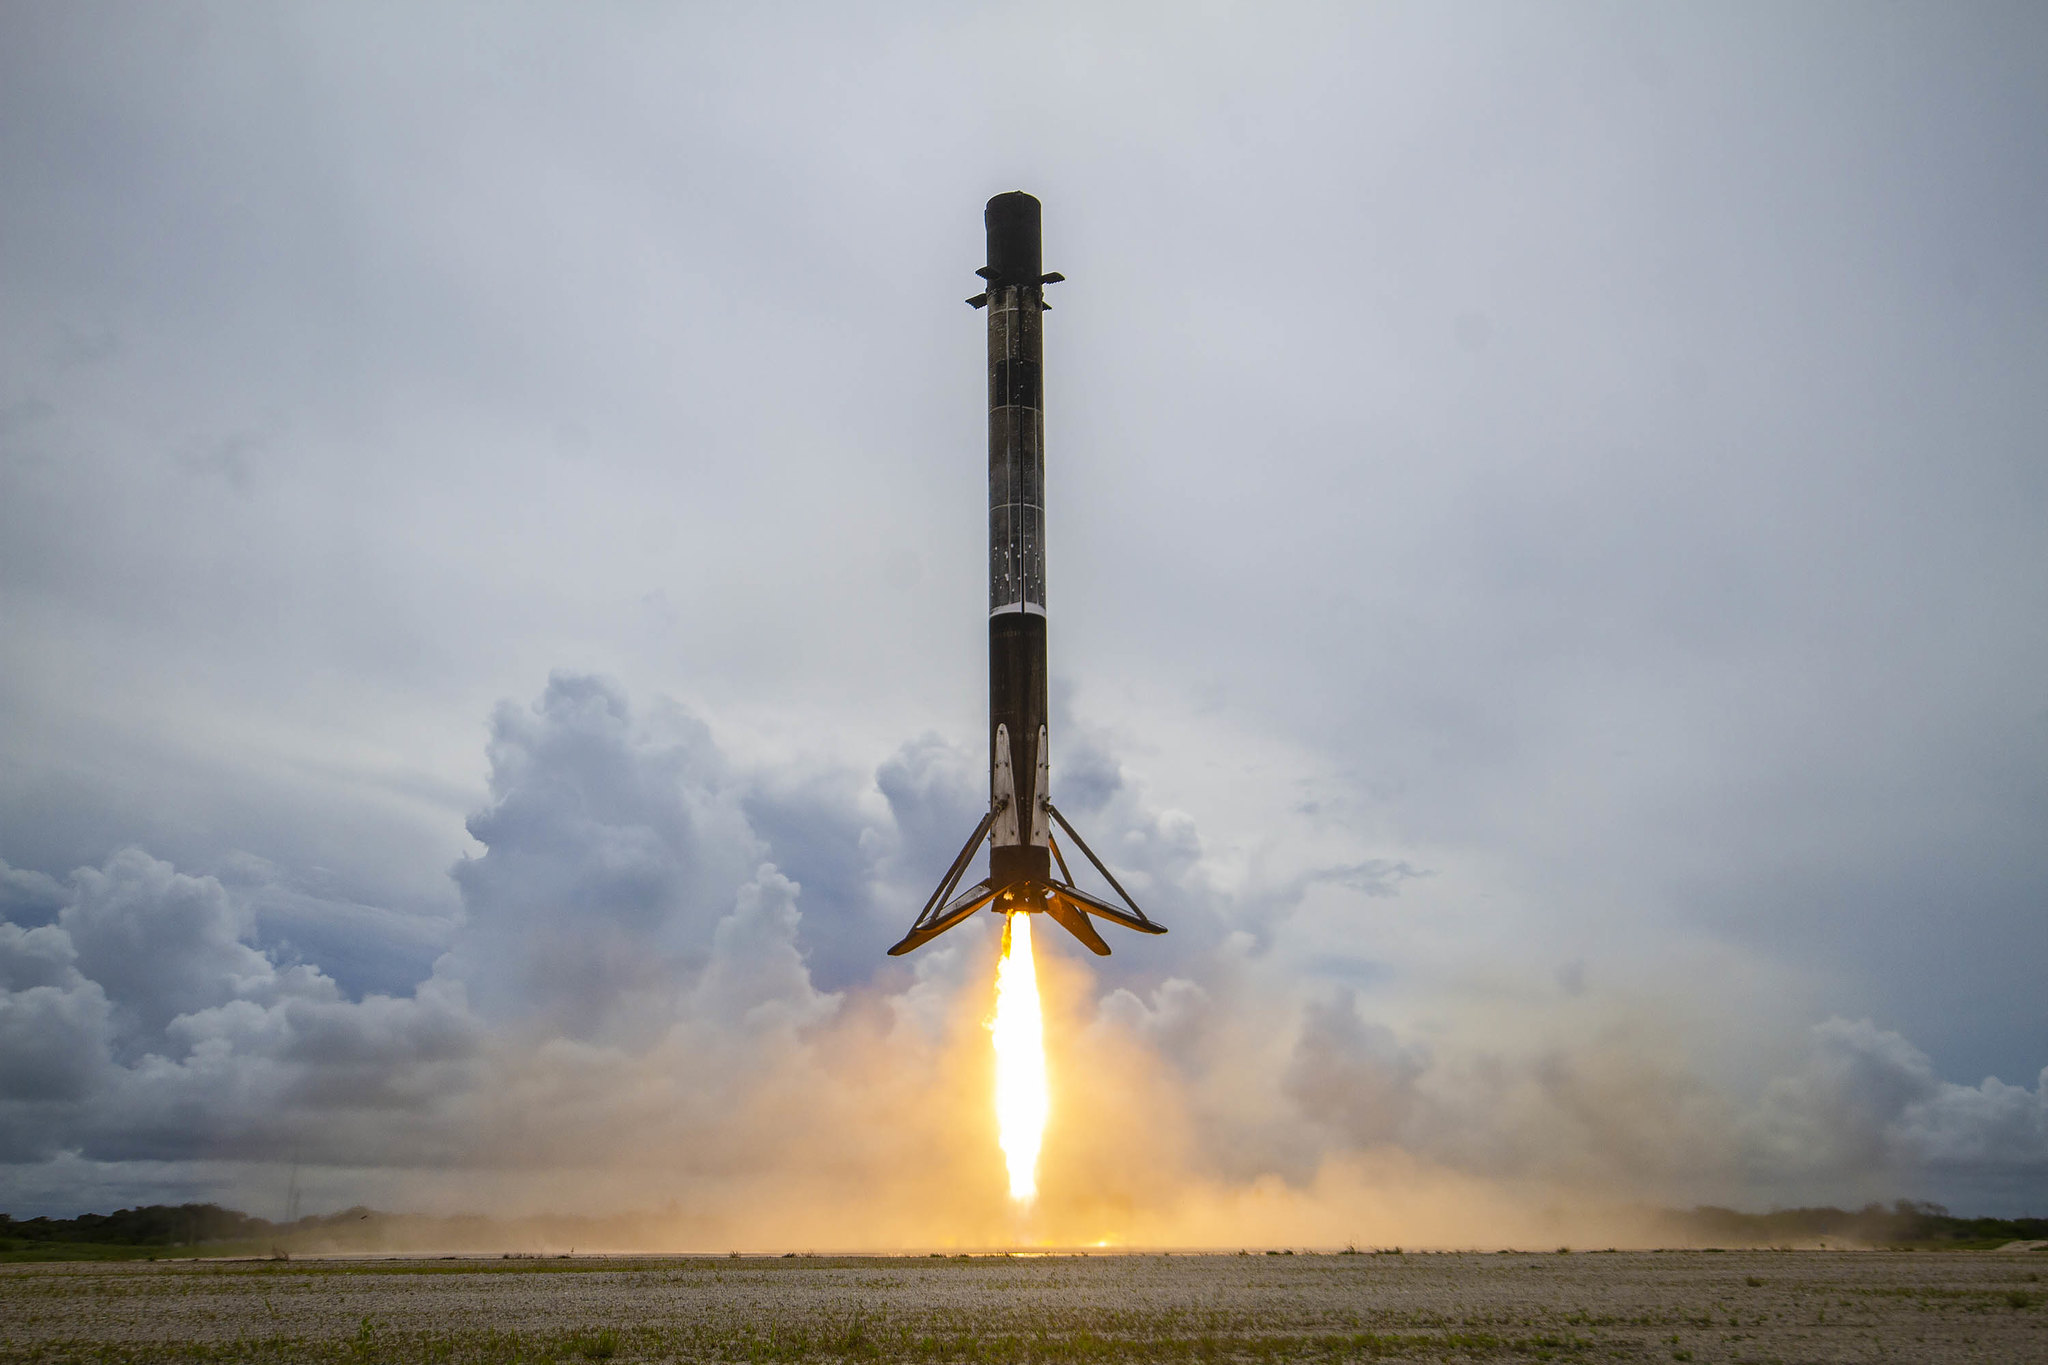
\includegraphics[width=0.68\linewidth]{Bilder/Falcon_9_Landung.jpg}
\end{center}
{\scriptsize Die erste Stufe einer Falcon-9-Rakete (SpaceX) kurz vor der
Landung.}

Nach dem Start fällt die erste Stufe einer Falcon-9-Rakete zurück Richtung
Erde, zunächst mit hoher und weiter zunehmender Geschwindigkeit. Kurz vor
der Landung zündet das Triebwerk erneut und bremst die Stufe ab, sodass
ihre Geschwindigkeit im Idealfall genau in dem Moment $v=0$ erreicht, in
dem sie den Boden berührt.

Die Ingenieurinnen und Ingenieure müssen im Voraus exakt berechnen, bei
welcher Höhe und mit welcher Bremsbeschleunigung das Triebwerk zünden
muss, damit Ort und Geschwindigkeit gleichzeitig null werden. Zündet das
Triebwerk zu spät oder zu schwach, ist die Stufe beim Aufsetzen noch zu
schnell und wird zerstört; zündet es zu früh oder zu stark, geht
wertvoller Treibstoff verloren. Genau solche Berechnungen ermöglichen die
Bewegungsgleichungen, die du in dieser Einheit herleitest.
\end{beispielbox}

% --- Einstieg: KEIN Rückgriff auf eine "Einfädelspuraufgabe" aus
% beschleunigung-arbeitsblatt.tex -- diese Übung (Rechteck+Dreieck,
% v0!=0) ist dort noch nicht umgesetzt, siehe Kommentar am Dateianfang.
% Stattdessen Anknüpfung an das, was dort TATSÄCHLICH schon steht: die
% Herleitung von s=1/2at^2 für den Spezialfall v0=0 ("Weg aus dem Stand").
% Als Recap zuerst nochmals die Skizze "Zwei Grundtypen der Bewegung im
% Vergleich" aus beschleunigung-arbeitsblatt.tex (dort ebenfalls mit
% $s$-Notation, deshalb unverändert übernommen -- diese Einheit bleibt
% durchgehend bei $s$, siehe Notation-Kommentar am Dateianfang). ---------
\begin{beispielbox}[Einstieg: Von Diagrammen zu Formeln]
Bisher hast du Bewegungen mit Diagrammen beschrieben: Bei einer
gleichförmigen Bewegung gilt $s=v\cdot t$, abgelesen als Fläche im
$v$-$t$-Diagramm. Im Beschleunigungsarbeitsblatt hast du für den
Spezialfall $v_0=0$ bereits $s=\tfrac12at^2$ hergeleitet, ebenfalls über
eine Fläche.

Jetzt verallgemeinern wir das: Mit den \textbf{\emph{Bewegungsgleichungen}}
lässt sich jede gleichförmige oder gleichmässig beschleunigte Bewegung
direkt mit einer Formel beschreiben und lösen, auch wenn $v_0\neq0$ oder
$s_0\neq0$ ist, ganz ohne Diagramm zeichnen zu müssen.

Erinnere dich zuerst an die zwei Grundtypen der Bewegung aus dem
Beschleunigungsarbeitsblatt:

\textbf{\emph{Gleichförmige Bewegung}} ($v=\text{konst.}$, also $a=0$):

\begin{center}
\begin{minipage}{0.30\linewidth}\centering
\begin{tikzpicture}[scale=0.62]
  \draw[->] (-0.3,0) -- (5,0) node[right] {\scriptsize $t$};
  \draw[->] (0,-0.3) -- (0,4.3) node[above] {\scriptsize $s$};
  \draw[thick,titleblue] (0,0) -- (4.5,3.6);
  \node[right] at (4.5,3.6) {\tiny $s=v\cdot t$};
\end{tikzpicture}\\[-0.2em]
{\scriptsize $s$-$t$: Gerade (Steigung $=v$)}
\end{minipage}\hfill
\begin{minipage}{0.30\linewidth}\centering
\begin{tikzpicture}[scale=0.62]
  \draw[->] (-0.3,0) -- (5,0) node[right] {\scriptsize $t$};
  \draw[->] (0,-0.3) -- (0,4.3) node[above] {\scriptsize $v$};
  \filldraw[lightblue] (0,0) rectangle (4.5,2.4);
  \draw[thick,titleblue] (0,2.4) -- (4.5,2.4);
  \draw[dashed,gray] (4.5,0) -- (4.5,2.4);
  \node at (2.25,2.75) {\tiny $v=\text{konst.}$};
  \node[align=center] at (2.25,1.2) {\tiny Fläche\\$=v\cdot t=s$};
\end{tikzpicture}\\[-0.2em]
{\scriptsize $v$-$t$: waagrecht}
\end{minipage}\hfill
\begin{minipage}{0.30\linewidth}\centering
\begin{tikzpicture}[scale=0.62]
  \draw[->] (-0.3,0) -- (5,0) node[right] {\scriptsize $t$};
  \draw[->] (0,-0.3) -- (0,4.3) node[above] {\scriptsize $a$};
  \draw[thick,titleblue] (0,0) -- (4.5,0);
  \node at (2.25,0.5) {\tiny $a=0$};
\end{tikzpicture}\\[-0.2em]
{\scriptsize $a$-$t$: auf der $t$-Achse ($a=0$)}
\end{minipage}
\end{center}

\textbf{\emph{Gleichmässig beschleunigte Bewegung}} ($a=\text{konst.}\neq0$):

\begin{center}
\begin{minipage}{0.30\linewidth}\centering
\begin{tikzpicture}[scale=0.62]
  \draw[->] (-0.3,0) -- (5,0) node[right] {\scriptsize $t$};
  \draw[->] (0,-0.3) -- (0,4.3) node[above] {\scriptsize $s$};
  \draw[thick,accentorange,domain=0:4.5,samples=60,smooth] plot (\x,{0.18*\x*\x});
  \node[right] at (4.5,3.65) {\tiny $s=\tfrac12at^2$};
\end{tikzpicture}\\[-0.2em]
{\scriptsize $s$-$t$: Parabel (immer steiler)}
\end{minipage}\hfill
\begin{minipage}{0.30\linewidth}\centering
\begin{tikzpicture}[scale=0.62]
  \draw[->] (-0.3,0) -- (5,0) node[right] {\scriptsize $t$};
  \draw[->] (0,-0.3) -- (0,4.3) node[above] {\scriptsize $v$};
  \filldraw[lightblue] (0,0) -- (4.5,3.6) -- (4.5,0) -- cycle;
  \draw[thick,accentorange] (0,0) -- (4.5,3.6);
  \draw[dashed,gray] (4.5,0) -- (4.5,3.6);
  \node[right] at (4.5,3.6) {\tiny $v=a\cdot t$};
  \node[align=center] at (3.15,0.9) {\tiny Fläche\\$=\tfrac12at^2=s$};
\end{tikzpicture}\\[-0.2em]
{\scriptsize $v$-$t$: Gerade (Steigung $=a$)}
\end{minipage}\hfill
\begin{minipage}{0.30\linewidth}\centering
\begin{tikzpicture}[scale=0.62]
  \draw[->] (-0.3,0) -- (5,0) node[right] {\scriptsize $t$};
  \draw[->] (0,-0.3) -- (0,4.3) node[above] {\scriptsize $a$};
  \filldraw[lightblue] (0,0) rectangle (4.5,2.4);
  \draw[thick,accentorange] (0,2.4) -- (4.5,2.4);
  \draw[dashed,gray] (4.5,0) -- (4.5,2.4);
  \node at (2.25,2.75) {\tiny $a=\text{konst.}$};
  \node[align=center] at (2.25,1.2) {\tiny Fläche\\$=a\cdot t=\Delta v$};
\end{tikzpicture}\\[-0.2em]
{\scriptsize $a$-$t$: waagrecht, aber $\neq0$}
\end{minipage}
\end{center}

Für beide Grundtypen leiten wir jetzt eine Formel her, mit der sich der
Ort direkt berechnen lässt, ohne ein Diagramm zeichnen zu müssen.
\end{beispielbox}

% =============================================================================
% Theorie: fachliche Grundlage für die Aufgaben, in eigene Boxen unterteilt
% (je Unterthema eine theoriebox), Reihenfolge = Lernzielreihenfolge oben.
% =============================================================================
\begin{theoriebox}[Gleichförmige Bewegung: von der Fläche zur Formel]
Bei einer gleichförmigen Bewegung ($v=\text{konst.}$) ist das
$v$-$t$-Diagramm eine waagrechte Linie. Die Fläche darunter, zwischen
$t_0$ und $t$, ist ein \textbf{\emph{Rechteck}} und entspricht wie immer
der zurückgelegten Strecke $\Delta s$:

\begin{center}
\begin{tikzpicture}[scale=0.85]
  \draw[->] (-0.3,0) -- (6.5,0) node[right] {\scriptsize $t$};
  \draw[->] (0,-0.3) -- (0,3.2) node[above] {\scriptsize $v$};
  \draw[dashed,gray] (0.6,0) -- (0.6,2.2);
  \draw[dashed,gray] (5.5,0) -- (5.5,2.2);
  \filldraw[lightblue] (0.6,0) rectangle (5.5,2.2);
  \draw[thick,titleblue] (0.6,2.2) -- (5.5,2.2);
  \draw (0.6,0.15) -- (0.6,-0.15) node[below] {\scriptsize $t_0$};
  \draw (5.5,0.15) -- (5.5,-0.15) node[below] {\scriptsize $t$};
  \node[left] at (0,2.2) {\scriptsize $v$};
  \node at (3,1.1) {\scriptsize Rechteck: $v\,(t-t_0)$};
\end{tikzpicture}
\end{center}

Fläche $=$ Höhe $\times$ Breite $=v\,(t-t_0)$. Zusammen mit dem Startort
$s_0$ ergibt das die \textbf{\emph{Ortsgleichung für gleichförmige
Bewegung}}:

\begin{formelbox}[Gleichförmige Bewegung]
\[
  v = \text{konstant}, \qquad s(t) = s_0 + v\,(t-t_0)
\]
Einheit von $s,s_0\colon\ \si{\meter}$.
\end{formelbox}

Nach $v$ aufgelöst (zum Beispiel um aus zwei Messpunkten die
Geschwindigkeit zu bestimmen):
\[
  v = \frac{s(t)-s_0}{t-t_0}.
\]

Im $s$-$t$-Diagramm ist das eine Gerade mit Achsenabschnitt $s_0$ und
Steigung $v$:

\begin{center}
\begin{tikzpicture}[scale=0.85]
  \draw[->] (-0.3,0) -- (6.5,0) node[right] {\scriptsize $t$};
  \draw[->] (0,-0.3) -- (0,4) node[above] {\scriptsize $s$};
  \draw[dashed,gray] (0,1) -- (0.7,1);
  \node[left] at (0,1) {\scriptsize $s_0$};
  \draw[thick,titleblue] (0.7,1) -- (5.7,3.6);
  \draw (0.7,0.15) -- (0.7,-0.15) node[below] {\scriptsize $t_0$};
  \filldraw[titleblue] (0.7,1) circle (1.4pt);
\end{tikzpicture}
\end{center}

\textbf{Beispiel:} Ein Zug fährt mit konstant
$v=\SI{100}{\kilo\meter\per\hour}$, Startort $s_0=0$. Nach
$t=\SI{2}{\hour}$: $s(2) = 0 + 100\cdot2 = \SI{200}{\kilo\meter}$.
\end{theoriebox}

\begin{questions}
\begin{taskbox}[Herleitung: Die Ortsgleichung aus der Fläche]
\question[6] Bei einer gleichmässig beschleunigten Bewegung
($a=\text{konst.}\neq0$) kennst du bereits die
\textbf{\emph{Geschwindigkeitsgleichung}} $v(t)=v_0+a(t-t_0)$: Zum
Zeitpunkt $t_0$ ist die Geschwindigkeit $v_0$, danach wächst (oder sinkt)
sie gleichmässig mit der Rate $a$. Im $v$-$t$-Diagramm ist das eine
Gerade. Die Fläche zwischen dieser Geraden und der $t$-Achse, zwischen
$t_0$ und $t$, zerfällt in zwei Teile:

\begin{center}
\begin{tikzpicture}[scale=0.85]
  \draw[->] (-0.3,0) -- (6.5,0) node[right] {\scriptsize $t$};
  \draw[->] (0,-0.3) -- (0,4) node[above] {\scriptsize $v$};
  \draw[thick,titleblue] (0.6,1.2) -- (5.5,3.4);
  \draw[dashed,gray] (0.6,0) -- (0.6,1.2);
  \draw[dashed,gray] (5.5,0) -- (5.5,3.4);
  \draw[dashed,gray] (0.6,1.2) -- (5.5,1.2);
  \filldraw[lightblue] (0.6,0) rectangle (5.5,1.2);
  \filldraw[verylightblue] (0.6,1.2) -- (5.5,1.2) -- (5.5,3.4) -- cycle;
  \draw (0.6,0.15) -- (0.6,-0.15) node[below] {\scriptsize $t_0$};
  \draw (5.5,0.15) -- (5.5,-0.15) node[below] {\scriptsize $t$};
  \node[left] at (0,1.2) {\scriptsize $v_0$};
  \node[left] at (-0.05,3.4) {\scriptsize $v(t)$};
  \node at (3,0.6) {\scriptsize Rechteck};
  \node at (4.55,2.1) {\scriptsize Dreieck};
\end{tikzpicture}
\end{center}

\begin{parts}
  \part[3] Bestimme $\Delta s$ als Summe von Rechteck- und Dreieckfläche,
  zunächst \textbf{\emph{nur mit $v_0$, $v(t)$, $t$ und $t_0$}} (setze
  $a$ noch nicht ein).
  \Antwortraum{3}
  \begin{solution}
  Rechteck (Höhe $v_0$, Breite $t-t_0$): Fläche $=v_0(t-t_0)$.\\
  Dreieck (Höhe $v(t)-v_0$, Breite $t-t_0$): Fläche
  $=\frac12\big(v(t)-v_0\big)(t-t_0)$.\\
  Zusammen:
  \[
    \Delta s = v_0(t-t_0) + \frac12\big(v(t)-v_0\big)(t-t_0).
  \]
  \end{solution}

  \part[3] Wir wissen bereits, dass $v(t)=v_0+a(t-t_0)$ gilt (siehe oben),
  also $v(t)-v_0=a(t-t_0)$. Setze das ein und vereinfache so weit wie
  möglich.
  \Antwortraum{3}
  \begin{solution}
  Einsetzen von $v(t)-v_0=a(t-t_0)$:
  \[
    \Delta s = v_0(t-t_0) + \frac12\,a(t-t_0)\,(t-t_0)
  \]
  Zusammenfassen:
  \[
    \Delta s = v_0(t-t_0) + \frac12\,a(t-t_0)^2.
  \]
  Mit $s(t)=s_0+\Delta s$ ist das genau die \textbf{\emph{Ortsgleichung}},
  die im Kasten unten festgehalten wird.
  \end{solution}
\end{parts}
\end{taskbox}
\end{questions}

\begin{theoriebox}[Gleichmässig beschleunigte Bewegung]
Addiert man zur Fläche aus der Übung oben noch den Startort $s_0$, erhält
man die \textbf{\emph{Ortsgleichung}}. Jeder Term hat eine feste
Bedeutung, die sich direkt im $s$-$t$-Diagramm wiederfindet:

\begin{center}
\begin{tikzpicture}[scale=0.85]
  \draw[->] (-0.3,0) -- (5.7,0) node[right] {\scriptsize $t$};
  \draw[->] (0,-0.3) -- (0,4.8) node[above] {\scriptsize $s$};
  \draw[thick,titleblue,domain=0:5,samples=60,smooth] plot (\x,{0.5+0.4*\x+0.08*\x*\x});
  \draw[dashed,gray] (0,0.5) -- (0.8,0.5);
  \node[left] at (0,0.5) {\scriptsize $s_0$};
  \filldraw[titleblue] (0,0.5) circle (1.4pt);
\end{tikzpicture}\\[0.2em]
{\scriptsize $s_0$: Startwert bei $t_0$ (Achsenabschnitt). $v_0$:
Anfangssteigung bei $t_0$. $a$: Krümmung der Parabel. Je grösser $|a|$,
desto stärker gekrümmt.}
\end{center}

Damit ergeben sich die drei wichtigsten Formeln dieser Einheit:

\begin{formelbox}[Gleichmässig beschleunigte Bewegung]
\[
  s(t) = s_0 + v_0(t-t_0) + \frac{1}{2}a(t-t_0)^2
\]
\[
  v(t) = v_0 + a\,(t-t_0)
\]
\[
  a(t) = a = \text{konst.}
\]
\end{formelbox}

\textbf{Beispiel:} Ein Auto startet bei einer Ampel
($v_0=\SI{0}{\meter\per\second}$, $s_0=\SI{0}{\meter}$) und beschleunigt
mit $a=\SI{2}{\meter\per\second\squared}$. Nach $t=\SI{3}{\second}$:
$v(3) = 0 + 2\cdot3 = \SI{6}{\meter\per\second}$ und
$s(3) = 0 + 0\cdot3 + \frac12\cdot2\cdot3^2 = \SI{9}{\meter}$.
\end{theoriebox}

\begin{questions}
\begin{taskbox}[Übung: Ortsgleichung anwenden]
\question[5] Ein Zug fährt mit $v_0=\SI{20}{\meter\per\second}$ und
bremst danach $\SI{8}{\second}$ lang konstant mit
$a=-\SI{1.5}{\meter\per\second\squared}$ (positive Richtung:
Fahrtrichtung, Startort $s_0=0$).

\begin{parts}
  \part[2] Zeichne dazu selbst ein $v$-$t$-Diagramm wie in der
  Theoriebox oben, mit eingezeichneter Rechteck- und
  Dreieckteilfläche.

  \begin{center}
  \begin{tikzpicture}[scale=0.85]
    \draw[->] (-0.3,0) -- (6.5,0) node[right] {\scriptsize $t$};
    \draw[->] (0,-0.3) -- (0,4) node[above] {\scriptsize $v$};
  \end{tikzpicture}
  \end{center}
  \begin{solution}
  \begin{center}
  \begin{tikzpicture}[scale=0.85]
    \draw[->] (-0.3,0) -- (6.5,0) node[right] {\scriptsize $t$};
    \draw[->] (0,-0.3) -- (0,4) node[above] {\scriptsize $v$};
    \draw[dashed,gray] (0.4,0) -- (0.4,3.4);
    \draw[dashed,gray] (5.2,0) -- (5.2,1.36);
    \draw[dashed,gray] (0.4,1.36) -- (5.2,1.36);
    \filldraw[lightblue] (0.4,0) rectangle (5.2,1.36);
    \filldraw[verylightblue] (0.4,1.36) -- (0.4,3.4) -- (5.2,1.36) -- cycle;
    \draw[thick,titleblue] (0.4,3.4) -- (5.2,1.36);
    \node[left] at (0,3.4) {\scriptsize $v_0$};
    \node[left] at (-0.05,1.36) {\scriptsize $v(t)$};
    \node at (2.8,0.7) {\scriptsize Rechteck};
    \node at (1.8,2.0) {\scriptsize Dreieck};
  \end{tikzpicture}
  \end{center}
  Da $a<0$ ist, liegt das Dreieck jetzt \emph{unterhalb} der
  $v_0$-Linie statt darüber: Die Geschwindigkeit nimmt ab, nicht zu.
  \end{solution}

  \part[3] Berechne die Position $s(8)$ direkt mit der Ortsgleichung von
  oben (nicht über die Flächen).
  \Antwortraum{3}
  \begin{solution}
  \[
    s(8) = s_0 + v_0\cdot t + \frac12\,a\,t^2
    = 0 + 20\cdot8 + \frac12\cdot(-1.5)\cdot8^2
  \]
  \[
    s(8) = 160 - 48 = \SI{112}{\meter}.
  \]
  \end{solution}
\end{parts}
\end{taskbox}
\end{questions}

% Übung wiederhergestellt aus der Git-Historie von v-t-diagramm-arbeitsblatt.tex
% (Commit a4876a3 entfernte die Teile c/d dieser Übung dort mit dem Kommentar
% "Die Fortsetzung mit Relativgeschwindigkeit/Überholmanöver gehört
% inhaltlich zum Thema Bewegungsgleichungen und lebt dort, nicht hier" --
% blieb aber bislang ungenutzt liegen; Bilder/Autos_Geschwindigkeit_Loesung.png
% lag deshalb schon in diesem Ordner. Teile a/b (Geschwindigkeiten
% umrechnen, Vektoren einzeichnen) bleiben im v-t-Diagramm-Arbeitsblatt, hier
% nur die Fortsetzung (Relativgeschwindigkeit, Überholmanöver), mit kurzem
% Recap der nötigen Werte. Teilaufgabe a) (Annäherungsphase) bleibt bei
% konstanten Geschwindigkeiten. Teilaufgabe b) (das eigentliche
% Überholmanöver) wurde nachträglich so umgebaut, dass das Auto während des
% Manövers beschleunigt statt konstant zu fahren -- dieselbe
% Ausgangssituation wie zuvor, jetzt aber mit Bewegungsgleichung statt
% Momentangeschwindigkeit gelöst. Die separate, unabhängige Übung
% "Überholmanöver mit Beschleunigung" weiter unten bleibt als eigenständiges,
% anspruchsvolleres Treffpunktproblem (zwei vollständige Ortsgleichungen,
% eigenes Koordinatensystem) bestehen.
\begin{questions}
\begin{taskbox}[Übung: Überholmanöver auf der Autobahn]
\question[9] Wiederholung aus dem $v$-$t$-Diagrammarbeitsblatt: Auf der
Autobahn (Höchstgeschwindigkeit $\SI{120}{\kilo\meter\per\hour}$) nähert
sich ein Auto mit $v_1=\SI{33.33}{\meter\per\second}$
($\approx\SI{120}{\kilo\meter\per\hour}$) einem Lastwagen mit
$v_2=\SI{22.22}{\meter\per\second}$ ($\approx\SI{80}{\kilo\meter\per\hour}$,
die für Lastwagen geltende Höchstgeschwindigkeit). Zum Zeitpunkt
$t=\SI{0}{\second}$ beträgt der Abstand zwischen den beiden Fahrzeugen
$d_0=\SI{70}{\meter}$ (siehe Bild). Der Lastwagen ist
$\ell_{\text{LKW}}=\SI{16.5}{\meter}$ lang (Länge eines modernen
Sattelzugs).

\begin{center}
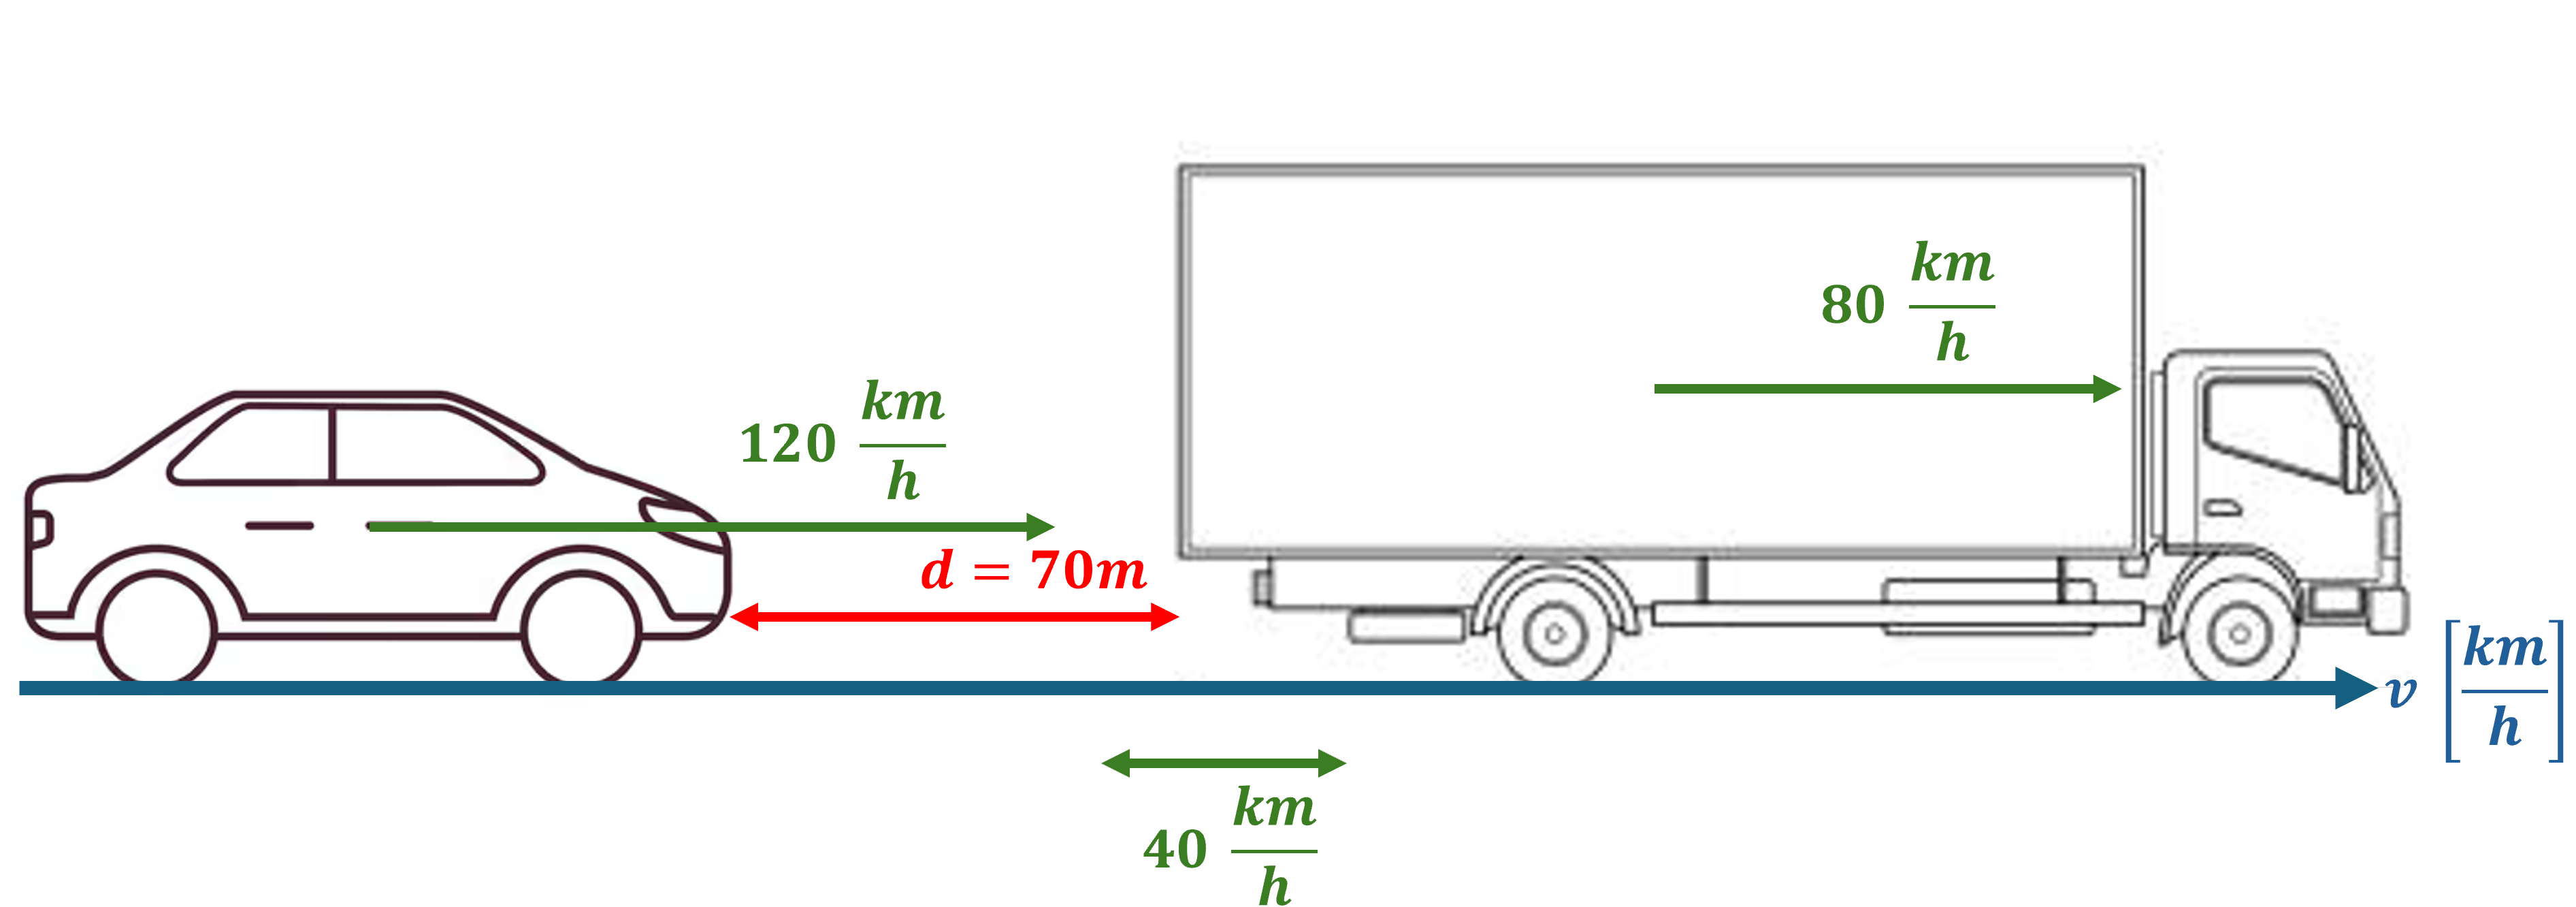
\includegraphics[width=0.75\linewidth]{Bilder/Autos_Geschwindigkeit_Loesung.png}
\end{center}

\begin{parts}
  \part[3] Das Auto will erst dann den Blinker setzen und mit dem
  Überholmanöver beginnen, wenn der Abstand zum Lastwagen auf
  $\SI{40}{\meter}$ Sicherheitsabstand geschrumpft ist. Nach welcher Zeit
  $t$ ist das der Fall?
  \Antwortraum{3}
  \begin{solution}
  Relativgeschwindigkeit: $v_1-v_2 \approx \SI{33.33}{\meter\per\second}
  - \SI{22.22}{\meter\per\second} = \SI{11.11}{\meter\per\second}$. Der
  Abstand muss dazu um $d_0-\SI{40}{\meter}=\SI{30}{\meter}$ abnehmen:
  \[
    t = \frac{\SI{30}{\meter}}{\SI{11.11}{\meter\per\second}}
    \approx \SI{2.70}{\second}.
  \]
  \end{solution}

  \part[6] Für das eigentliche Überholmanöver (auf der Überholspur)
  bleiben dem Auto nur $\SI{6}{\second}$, weil sich von hinten bereits
  ein schnelleres Fahrzeug nähert und die Spur zügig wieder freigegeben
  werden muss. Danach soll das Auto $\SI{30}{\meter}$ Vorsprung vor dem
  Lastwagen haben. Berücksichtige dabei, dass das Auto nicht nur die
  $\SI{40}{\meter}$ Sicherheitsabstand aufholen muss, sondern zusätzlich
  die ganze Länge $\ell_{\text{LKW}}$ des Lastwagens überholen muss, bevor
  es wieder auf die rechte Spur einschwenken kann. Statt konstant
  weiterzufahren, tritt das Auto zu Beginn des Manövers aufs Gaspedal und
  beschleunigt von da an mit konstanter Beschleunigung $a$ (Startgeschwindigkeit
  weiterhin $v_1$), während der Lastwagen unverändert mit $v_2$
  weiterfährt. Mit welcher Beschleunigung $a$ muss das Auto mindestens
  beschleunigen, damit es den nötigen Vorsprung rechtzeitig erreicht?
  Berechne ausserdem, welche Geschwindigkeit das Auto am Ende des
  Manövers erreicht (in $\si{\meter\per\second}$ \emph{und} in
  $\si{\kilo\meter\per\hour}$).
  \Antwortraum{6}
  \begin{solution}
  Zu Beginn des Manövers liegt das Auto noch $\SI{40}{\meter}$ zurück
  (Front Auto zu Heck Lastwagen). Bis es wieder einschwenken kann, muss es
  zusätzlich die ganze Lastwagenlänge $\ell_{\text{LKW}}=\SI{16.5}{\meter}$
  aufholen, und danach soll es $\SI{30}{\meter}$ Vorsprung haben: Relativ
  zum Lastwagen muss es also
  $\SI{40}{\meter}+\SI{16.5}{\meter}+\SI{30}{\meter}=\SI{86.5}{\meter}$
  aufholen, und zwar in $\SI{6}{\second}$.

  Im mitbewegten Bezugssystem des Lastwagens (der selbst konstant mit
  $v_2$ weiterfährt) startet das Auto mit der Relativgeschwindigkeit
  $v_1-v_2\approx\SI{11.11}{\meter\per\second}$ (aus Teilaufgabe a) und
  beschleunigt von da an mit $a$. Die relative Strecke folgt also der
  Ortsgleichung $\Delta s_{\text{rel}} = (v_1-v_2)\,t+\frac12 a t^2$:
  \[
    \SI{86.5}{\meter} = \SI{11.11}{\meter\per\second}\cdot\SI{6}{\second} + \frac12\,a\cdot(\SI{6}{\second})^2.
  \]
  Rechte Seite ausrechnen ($11.11\cdot6=66.66$, $\frac12\cdot6^2=18$):
  \[
    \SI{86.5}{\meter} = \SI{66.66}{\meter} + a\cdot\SI{18}{\second\squared}.
  \]
  Auf beiden Seiten $-\SI{66.66}{\meter}$:
  \[
    \SI{19.84}{\meter} = a\cdot\SI{18}{\second\squared}.
  \]
  Auf beiden Seiten durch $\SI{18}{\second\squared}$ teilen:
  \[
    a \approx \SI{1.10}{\meter\per\second\squared}.
  \]
  Geschwindigkeit am Ende des Manövers (mit dem noch nicht gerundeten Wert
  $a\approx\SI{1.1022}{\meter\per\second\squared}$ weitergerechnet, damit
  sich der Rundungsfehler nicht aufsummiert):
  \[
    v_{\text{ende}} = v_1 + a\cdot t \approx \SI{33.33}{\meter\per\second}
    + \SI{1.1022}{\meter\per\second\squared}\cdot\SI{6}{\second}
    \approx \SI{39.94}{\meter\per\second} \approx \SI{143.8}{\kilo\meter\per\hour}.
  \]
  \textbf{Hinweis:} Weil das Auto das Manöver mit seiner
  Ausgangsgeschwindigkeit $v_1$ beginnt (also langsamer als die nötige
  Durchschnittsgeschwindigkeit), muss es am Ende sogar noch schneller
  fahren als die rund $\SI{131.9}{\kilo\meter\per\hour}$, die bei
  konstanter Geschwindigkeit während des ganzen Manövers nötig wären. Das
  Manöver bleibt also auch mit Beschleunigung deutlich ausserhalb der
  erlaubten Autobahnhöchstgeschwindigkeit von $\SI{120}{\kilo\meter\per\hour}$
  und ist im gegebenen Zeitfenster nicht regelkonform durchführbar.
  \end{solution}
\end{parts}
\end{taskbox}
\end{questions}

% Theorie zur quadratischen Funktion: keine Ableitung (noch nicht
% bekannt), Farbcodierung der Komponenten (s_0/C = titleblue, v_0/B =
% accentorange, a/A = accentpurple) statt nur Buchstaben, keine Tangente
% im Diagramm.
\begin{theoriebox}[Was ist eine Parabel? Die quadratische Funktion]
Bevor wir weiterrechnen, ein kurzer Blick auf die Mathematik hinter der
Ortsgleichung. Eine Funktion der Form
\[
  f(t) = \textcolor{accentpurple}{A}\,t^2 + \textcolor{accentorange}{B}\,t + \textcolor{titleblue}{C}
\]
heisst \textbf{\emph{quadratische Funktion}} (weil $t$ im Quadrat
vorkommt), und ihr Graph heisst \textbf{\emph{Parabel}}. Die drei
Koeffizienten haben jeweils eine feste Bedeutung:
\begin{itemize}[leftmargin=1.2cm,itemsep=0.25em]
  \item \textcolor{titleblue}{$C$}: der Funktionswert bei $t=0$ (wo die
  Parabel die senkrechte Achse schneidet).
  \item \textcolor{accentorange}{$B$}: die \textbf{\emph{Anfangssteigung}}
  bei $t=0$.
  \item \textcolor{accentpurple}{$A$}: bestimmt die
  \textbf{\emph{Krümmung}} der Parabel: Sie öffnet sich nach oben, wenn
  $A>0$ ist, und nach unten, wenn $A<0$ ist.
\end{itemize}

Vergleiche das jetzt mit der Ortsgleichung (mit $t_0=0$):
\[
  s(t) = \underbrace{\textcolor{titleblue}{s_0}}_{C} + \underbrace{\textcolor{accentorange}{v_0}}_{B}\,t + \underbrace{\textcolor{accentpurple}{\tfrac{1}{2}a}}_{A}\,t^2.
\]
Die Ortsgleichung ist also genau von dieser Form, mit $C=s_0$, $B=v_0$
und $A=\frac{1}{2}a$:
\begin{itemize}[leftmargin=1.2cm,itemsep=0.25em]
  \item \textcolor{titleblue}{$s_0$} (der Startort) entspricht $C$: dem
  Wert von $s(t)$ bei $t=0$.
  \item \textcolor{accentorange}{$v_0$} (die Startgeschwindigkeit)
  entspricht $B$: der Anfangssteigung der Parabel.
  \item \textcolor{accentpurple}{$\frac{1}{2}a$} entspricht $A$: Die
  Beschleunigung $a$ bestimmt also, wie stark sich die Parabel krümmt und
  in welche Richtung sie sich öffnet (nach oben bei $a>0$, nach unten bei
  $a<0$).
\end{itemize}
Sobald $a\neq0$ ist, taucht $t$ im Quadrat auf, und $s(t)$ ist deshalb
zwangsläufig eine Parabel. Nur wenn $a=0$ ist (gleichförmige Bewegung),
bleibt der quadratische Term weg, und $s(t)$ wird zu einer Geraden.

Als konkretes Zahlenbeispiel: $f(t) = 0.15\,t^2 + 0.6\,t + 0.5$, also
$\textcolor{accentpurple}{A=0.15}$, $\textcolor{accentorange}{B=0.6}$,
$\textcolor{titleblue}{C=0.5}$.

\begin{center}
\begin{tikzpicture}[scale=0.8]
  \draw[->] (-0.3,0) -- (4,0) node[right] {\scriptsize $t$};
  \draw[->] (0,-0.3) -- (0,4.6) node[above] {\scriptsize $s$};
  \draw[thick,titleblue,domain=0:3.4,samples=60,smooth] plot (\x,{0.15*\x*\x+0.6*\x+0.5});
  \draw[dashed,gray] (0,0.5) -- (0.5,0.5);
  \node[left] at (0,0.5) {\scriptsize $C=s_0=0.5$};
  \filldraw[titleblue] (0,0.5) circle (1.4pt);
\end{tikzpicture}\\[0.2em]
{\scriptsize Graph von $f(t)=0.15\,t^2+0.6\,t+0.5$.}
\end{center}
\end{theoriebox}

\begin{theoriebox}[Vom s-t- zum v-t-Diagramm (und zurück)]
Wie du beim Beschleunigungsarbeitsblatt gesehen hast, gehört zu einer
gleichmässig beschleunigten Bewegung eine $s$-$t$-Parabel und ein
\textbf{\emph{lineares}} $v$-$t$-Diagramm. Der Zusammenhang: $v(t)$
entspricht der \textbf{\emph{Steigung}} der Parabel an jeder Stelle. Drei
Übersetzungsregeln reichen, um qualitativ (ohne Rechnung) zwischen beiden
Diagrammen hin- und herzuwechseln:
\begin{itemize}[leftmargin=1.2cm,itemsep=0.25em]
  \item Die \textbf{\emph{Anfangssteigung}} der Parabel bei $t_0$ entspricht der \textbf{\emph{Starthöhe}} $v_0$ der Geraden.
  \item Der \textbf{\emph{Scheitelpunkt}} der Parabel (waagrechte Tangente) entspricht der \textbf{\emph{Nullstelle}} der Geraden ($v=0$).
  \item Öffnet sich die Parabel nach \textbf{\emph{oben}} ($a>0$), ist die Gerade \textbf{\emph{steigend}}; öffnet sie sich nach \textbf{\emph{unten}} ($a<0$), ist die Gerade \textbf{\emph{fallend}}.
\end{itemize}

\begin{center}
\begin{minipage}{0.47\linewidth}\centering
\begin{tikzpicture}[scale=0.75]
  \draw[->] (-0.3,0) -- (5,0) node[right] {\scriptsize $t$};
  \draw[->] (0,-0.3) -- (0,3.6) node[above] {\scriptsize $s$};
  \draw[thick,titleblue,domain=0:4.3,samples=60,smooth] plot (\x,{0.28*(\x-2.2)*(\x-2.2)+0.3});
  \draw[dashed,gray] (2.2,0) -- (2.2,0.3);
  \draw (2.2,0.15) -- (2.2,-0.15) node[below] {\scriptsize $t^\ast$};
\end{tikzpicture}\\[-0.2em]
{\scriptsize $s(t)$: Parabel, Scheitel bei $t^\ast$}
\end{minipage}\hfill
\begin{minipage}{0.47\linewidth}\centering
\begin{tikzpicture}[scale=0.75]
  \draw[->] (-0.3,0) -- (5,0) node[right] {\scriptsize $t$};
  \draw[->] (0,-1.6) -- (0,1.8) node[above] {\scriptsize $v$};
  \draw[thick,titleblue] (0,-1.4) -- (4.4,1.4);
  \draw[dashed,gray] (2.2,0) -- (2.2,-1.6);
  \draw (2.2,0.15) -- (2.2,-0.15) node[below] {\scriptsize $t^\ast$};
\end{tikzpicture}\\[-0.2em]
{\scriptsize $v(t)$: Gerade, Nullstelle bei $t^\ast$}
\end{minipage}
\end{center}
\end{theoriebox}

\begin{questions}
\begin{taskbox}[Übung: Zwischen s(t) und v(t) übersetzen]
\question[6]
\begin{parts}
  \part[3] Gegeben ist $s(t) = 2+4t+t^2$ (in $\si{\meter}$, $t$ in $\si{\second}$).
  Lies $v_0$ und $a$ direkt aus dieser Gleichung ab (Vergleich mit
  $s(t)=s_0+v_0t+\frac{1}{2}at^2$) und skizziere $v(t)$ qualitativ (ohne
  Achsenbeschriftung mit Zahlen, nur Startpunkt, Steigung und Vorzeichen
  müssen stimmen).

  \begin{center}
  \begin{tikzpicture}[scale=0.85]
    \draw[->] (-0.3,0) -- (4.5,0) node[right] {\scriptsize $t$};
    \draw[->] (0,-0.3) -- (0,3.3) node[above] {\scriptsize $v$};
  \end{tikzpicture}
  \end{center}
  \begin{solution}
  Vergleich: $v_0=4$, $\frac{1}{2}a=1\Rightarrow a=2$. Also
  $v(t)=4+2t$: eine steigende Gerade, die bei $v_0=4$ startet.
  \begin{center}
  \begin{tikzpicture}[scale=0.85]
    \draw[->] (-0.3,0) -- (4.5,0) node[right] {\scriptsize $t$};
    \draw[->] (0,-0.3) -- (0,3.3) node[above] {\scriptsize $v$};
    \draw[thick,titleblue] (0,1) -- (4,3);
    \node[left] at (0,1) {\scriptsize $v_0$};
  \end{tikzpicture}
  \end{center}
  \end{solution}

  \part[3] Gegeben ist $v(t) = 8-2t$ (in $\si{\meter\per\second}$, $t$ in
  $\si{\second}$). Skizziere $s(t)$ qualitativ: Achte auf die Anfangssteigung,
  die Öffnungsrichtung und die Lage des Scheitelpunkts.

  \begin{center}
  \begin{tikzpicture}[scale=0.85]
    \draw[->] (-0.3,0) -- (4.5,0) node[right] {\scriptsize $t$};
    \draw[->] (0,-0.3) -- (0,3.3) node[above] {\scriptsize $s$};
  \end{tikzpicture}
  \end{center}
  \begin{solution}
  $v_0=8>0$ (Parabel startet mit steiler positiver Steigung), $a=-2<0$
  (Parabel öffnet sich nach unten). Nullstelle von $v(t)$ bei $t=4$, also
  liegt dort der Scheitelpunkt (Maximum) der Parabel.
  \begin{center}
  \begin{tikzpicture}[scale=0.85]
    \draw[->] (-0.3,0) -- (4.5,0) node[right] {\scriptsize $t$};
    \draw[->] (0,-0.3) -- (0,3.3) node[above] {\scriptsize $s$};
    \draw[thick,titleblue,domain=0:4.3,samples=60,smooth] plot (\x,{-0.19*(\x-4)*(\x-4)+3.2});
    \draw[dashed,gray] (4,0) -- (4,3.2);
    \draw (4,0.15) -- (4,-0.15) node[below] {\scriptsize $t=4$};
  \end{tikzpicture}
  \end{center}
  \end{solution}
\end{parts}
\end{taskbox}
\end{questions}

\begin{questions}
\begin{taskbox}[Übung: Mittlere Geschwindigkeit aus dem v-t-Diagramm]
\question[7] Ein Velofahrer fährt mit $v_0=\SI{5}{\meter\per\second}$ und
beschleunigt danach $\SI{8}{\second}$ lang gleichmässig auf
$v=\SI{15}{\meter\per\second}$.

\begin{parts}
  \part[1] Zeichne das $v$-$t$-Diagramm dieser Bewegung (Gerade von $v_0$
  nach $v$) und schraffiere die Fläche darunter.

  \begin{center}
  \begin{tikzpicture}[scale=0.85]
    \draw[->] (-0.3,0) -- (6.5,0) node[right] {\scriptsize $t$ in s};
    \draw[->] (0,-0.3) -- (0,4.3) node[above] {\scriptsize $v$ in $\si{\meter\per\second}$};
  \end{tikzpicture}
  \end{center}
  \begin{solution}
  \begin{center}
  \begin{tikzpicture}[scale=0.85]
    \draw[->] (-0.3,0) -- (6.5,0) node[right] {\scriptsize $t$ in s};
    \draw[->] (0,-0.3) -- (0,4.3) node[above] {\scriptsize $v$ in $\si{\meter\per\second}$};
    \filldraw[lightblue] (0,0) -- (0,1.25) -- (5.5,3.75) -- (5.5,0) -- cycle;
    \draw[thick,titleblue] (0,1.25) -- (5.5,3.75);
    \draw[dashed,gray] (5.5,0) -- (5.5,3.75);
    \node[left] at (0,1.25) {\scriptsize $v_0$};
    \node[left] at (-0.05,3.75) {\scriptsize $v$};
    \draw (5.5,0.15) -- (5.5,-0.15) node[below] {\scriptsize $t$};
  \end{tikzpicture}
  \end{center}
  \end{solution}

  \part[2] Zeige: Die Fläche unter dieser Geraden (ein Trapez) ist genau
  so gross wie die Fläche eines Rechtecks mit derselben Breite $\Delta t$
  und der Höhe $\bar v=\dfrac{v_0+v}{2}$, der \textbf{\emph{mittleren
  Geschwindigkeit}}. Begründe kurz, weshalb das bei einer
  \emph{geraden} Linie im $v$-$t$-Diagramm immer funktioniert, bei einer
  gekrümmten Kurve aber nicht mehr.
  \Antwortraum{2}
  \begin{solution}
  Das Trapez lässt sich wie gewohnt in ein Rechteck der Höhe $v_0$ und
  ein Dreieck der Höhe $v-v_0$ zerlegen. Ein Rechteck der Höhe
  $\bar v=\frac{v_0+v}{2}$ über derselben Breite $\Delta t$ hat exakt
  dieselbe Fläche, weil das Dreieck genau die Fläche ausgleicht, die dem
  Rechteck der Höhe $\bar v$ oben fehlt bzw.\ die es unten zu viel hat.
  Das funktioniert nur, weil die Linie \emph{gerade} ist (konstante
  Steigung, also konstantes $a$): Bei einer gekrümmten Kurve (nicht
  konstantes $a$) liegt der Mittelwert der beiden Randwerte nicht mehr
  auf der Kurve, und die Flächen stimmen nicht mehr überein.
  \end{solution}

  \part[2] Berechne mit der mittleren Geschwindigkeit $\bar v$ die in
  diesen $\SI{8}{\second}$ zurückgelegte Strecke $\Delta s=\bar
  v\cdot\Delta t$.
  \Antwortraum{2}
  \begin{solution}
  \[
    \bar v = \frac{v_0+v}{2} = \frac{\SI{5}{\meter\per\second}+\SI{15}{\meter\per\second}}{2} = \SI{10}{\meter\per\second}.
  \]
  \[
    \Delta s = \bar v\cdot\Delta t = \SI{10}{\meter\per\second}\cdot\SI{8}{\second} = \SI{80}{\meter}.
  \]
  \end{solution}

  \part[2] Berechne dieselbe Strecke jetzt mit der Ortsgleichung
  $s(t)=s_0+v_0(t-t_0)+\frac12a(t-t_0)^2$ (bestimme zuerst $a$ mit der
  Geschwindigkeitsgleichung), und vergleiche mit Teilaufgabe c).
  \Antwortraum{2}
  \begin{solution}
  \[
    a = \frac{v-v_0}{\Delta t} = \frac{\SI{15}{\meter\per\second}-\SI{5}{\meter\per\second}}{\SI{8}{\second}} = \SI{1.25}{\meter\per\second\squared}.
  \]
  \[
    \Delta s = v_0\,\Delta t + \frac12 a\,\Delta t^2 = 5\cdot8 + \frac12\cdot1.25\cdot8^2 = 40+40 = \SI{80}{\meter}.
  \]
  Exakt dasselbe Ergebnis wie mit der mittleren Geschwindigkeit: Bei
  gleichmässig beschleunigter Bewegung führen beide Wege zum selben
  Resultat, der Weg über $\bar v$ ist aber oft schneller gerechnet.
  \end{solution}
\end{parts}
\end{taskbox}
\end{questions}

\begin{theoriebox}[Die dritte Bewegungsgleichung: ohne die Zeit]
Manchmal ist die Zeit $t$ weder gegeben noch gesucht, zum Beispiel wenn
du nur wissen willst, wie schnell ein Objekt nach einer bestimmten
Strecke ist. Dafür gibt es eine dritte Gleichung, die $t$ gar nicht
enthält. Wir leiten sie in kleinen Schritten her.

\textbf{Schritt 1:} Die Geschwindigkeitsgleichung $v(t)=v_0+a(t-t_0)$
nach $(t-t_0)$ auflösen:
\[
  v - v_0 = a(t-t_0)
  \quad\Longrightarrow\quad
  t-t_0 = \frac{v-v_0}{a}.
\]

\textbf{Schritt 2:} Das in die Ortsgleichung
$\Delta s = v_0(t-t_0)+\frac{1}{2}a(t-t_0)^2$ einsetzen:
\[
  \Delta s = v_0\cdot\frac{v-v_0}{a} + \frac{1}{2}a\left(\frac{v-v_0}{a}\right)^2.
\]

\textbf{Schritt 3:} Den Bruch im zweiten Term quadrieren
($\left(\frac{v-v_0}{a}\right)^2 = \frac{(v-v_0)^2}{a^2}$) und kürzen
($\frac{1}{2}a\cdot\frac{1}{a^2}=\frac{1}{2a}$):
\[
  \Delta s = \frac{v_0(v-v_0)}{a} + \frac{(v-v_0)^2}{2a}.
\]

\textbf{Schritt 4:} Beide Brüche auf den gemeinsamen Nenner $2a$ bringen
(dazu den ersten Bruch mit $2$ erweitern):
\[
  \Delta s = \frac{2v_0(v-v_0)}{2a} + \frac{(v-v_0)^2}{2a}
  = \frac{2v_0(v-v_0) + (v-v_0)^2}{2a}.
\]

\textbf{Schritt 5:} Im Zähler $(v-v_0)$ ausklammern:
\[
  2v_0(v-v_0) + (v-v_0)^2 = (v-v_0)\,\big[2v_0 + (v-v_0)\big] = (v-v_0)(v+v_0).
\]

\textbf{Schritt 6:} Das ist die binomische Formel rückwärts angewendet
($(v-v_0)(v+v_0)=v^2-v_0^2$), also:
\[
  \Delta s = \frac{v^2-v_0^2}{2a}.
\]

\textbf{Schritt 7:} Mit $2a$ multiplizieren und nach $v^2$ umstellen:
\[
  2a\,\Delta s = v^2-v_0^2
  \quad\Longrightarrow\quad
  v^2 = v_0^2 + 2a\,\Delta s.
\]

Das ist die \textbf{\emph{zeitfreie Bewegungsgleichung}}:

\begin{formelbox}[Bewegungsgleichung 3: ohne die Zeit]
\[
  \boxed{v^2 = v_0^2 + 2a\,\Delta s}, \qquad \Delta s = s-s_0.
\]
\textbf{Beispiel:} Ein Flugzeug startet mit $v_0=\SI{0}{\meter\per\second}$
und beschleunigt konstant mit $a=\SI{3}{\meter\per\second\squared}$.
Welche Geschwindigkeit hat es nach $\Delta s=\SI{600}{\meter}$
Startbahn? $v^2 = 0 + 2\cdot3\cdot600 = 3600\,\si{\meter\squared\per\second\squared}
\Rightarrow v=\SI{60}{\meter\per\second}$.
\end{formelbox}
\end{theoriebox}

\begin{anleitungbox}[Wie wähle ich die passende Bewegungsgleichung?]
Bei jeder Aufgabe hilft dieselbe kleine Checkliste, um die richtige
Gleichung zu finden:

\begin{enumerate}[leftmargin=1.2cm,itemsep=0.3em]
  \item \textbf{\emph{Ist die Bewegung überhaupt beschleunigt?}} Steht in
  der Aufgabe $a=0$ (oder \glqq konstante Geschwindigkeit\grqq{})? Dann
  reicht die Gleichung für gleichförmige Bewegung
  ($s(t)=s_0+v(t-t_0)$), fertig.
  \item Falls $a\neq0$ ist: \textbf{\emph{Was ist gegeben, was ist
  gesucht?}} Schreibe dir zuerst alle gegebenen Grössen auf
  ($s_0$, $v_0$, $a$, $t$, $s$ oder $v$) und markiere, welche gesucht
  ist.
  \item \textbf{\emph{Welche Gleichung passt zu deiner Liste?}} Gehe die
  drei Gleichungen in der Tabelle unten der Reihe nach durch und
  vergleiche sie mit deiner Liste aus Schritt 2: Kommen in einer Gleichung
  nur Grössen vor, die entweder gegeben sind oder genau die gesuchte
  Grösse? Sobald das der Fall ist, hast du die richtige Gleichung
  gefunden, denn sie lässt sich sofort nach der gesuchten Grösse auflösen,
  ohne dass du vorher eine andere unbekannte Grösse berechnen müsstest.
\end{enumerate}

\begin{center}
{\small
\setlength{\tabcolsep}{4pt}
\begin{tabular}{p{7.6cm}p{2.6cm}p{3.7cm}}
\toprule
\textbf{Gleichung} & \textbf{Enthält} & \textbf{Wähle sie, wenn \dots} \\
\midrule
$v(t)=v_0+a(t-t_0)$ & $v,v_0,a,t$ & der Ort keine Rolle spielt \\[0.3em]
$s(t)=s_0+v_0(t-t_0)+\frac{1}{2}a(t-t_0)^2$ & $s,s_0,v_0,a,t$ & sowohl Ort als auch Zeit vorkommen \\[0.3em]
$v^2=v_0^2+2a\Delta s$ & $v,v_0,a,\Delta s$ & die Zeit weder gegeben noch gesucht ist \\
\bottomrule
\end{tabular}
}
\end{center}

\textbf{Beispiel:} Ein Auto ($s_0=0$, $v_0=\SI{10}{\meter\per\second}$)
beschleunigt konstant mit $a=\SI{2}{\meter\per\second\squared}$. Gesucht
ist seine Geschwindigkeit, nachdem es $\Delta s=\SI{100}{\meter}$
zurückgelegt hat.
\begin{enumerate}[leftmargin=1.2cm,itemsep=0.25em]
  \item $a=\SI{2}{\meter\per\second\squared}\neq0$: Die Bewegung ist
  beschleunigt, die Gleichung für gleichförmige Bewegung reicht nicht.
  \item Gegeben: $s_0$, $v_0$, $a$, $\Delta s$. Gesucht: $v$. Die Zeit $t$
  kommt in der Aufgabe gar nicht vor.
  \item Nur Bewegungsgleichung 3 enthält $v,v_0,a,\Delta s$ ohne $t$: also
  $v^2=v_0^2+2a\Delta s = 10^2+2\cdot2\cdot100 = 500 \Rightarrow
  v=\sqrt{500}\approx\SI{22.4}{\meter\per\second}$.
\end{enumerate}
\end{anleitungbox}

\begin{beispielbox}[Beispiel: E-Trottinett bremst]
Ein E-Trottinett ist mit $v_0=\SI{6}{\meter\per\second}$ unterwegs (die
positive Richtung sei die Fahrtrichtung) und bremst danach konstant mit
$a=-\SI{2}{\meter\per\second\squared}$, bis es steht.

\textbf{Welche Formel?} Gesucht ist die Bremsstrecke $\Delta s$. Gegeben
sind $v_0$, $a$ und die Endgeschwindigkeit $v=0$ (beim Stillstand). Die
Zeit ist weder gegeben noch gesucht, also ist $v^2=v_0^2+2a\Delta s$ die
richtige Wahl, nicht die Ortsgleichung (die würde zusätzlich die
unbekannte Bremszeit $t$ enthalten).

Werte einsetzen und $2\cdot(-2)=-4$ zusammenfassen:
\[
  0 = \SI{36}{\meter\squared\per\second\squared} - \SI{4}{\meter\per\second\squared}\cdot\Delta s.
\]
Auf beiden Seiten $+4\,\si{\meter\per\second\squared}\cdot\Delta s$ addieren:
\[
  \SI{4}{\meter\per\second\squared}\cdot\Delta s = \SI{36}{\meter\squared\per\second\squared}.
\]
Auf beiden Seiten durch $\SI{4}{\meter\per\second\squared}$ teilen:
\[
  \Delta s = \frac{36\,\si{\meter\squared\per\second\squared}}{4\,\si{\meter\per\second\squared}} = \SI{9}{\meter}.
\]

\textbf{Zum Vorzeichen:} Obwohl das Trottinett die ganze Zeit vorwärts
(also in die \emph{positive} Richtung) fährt, ist $a$ \emph{negativ}. Das
ist kein Widerspruch: $a<0$ heisst nicht \glqq bewegt sich rückwärts\grqq{},
sondern \glqq $a$ zeigt in die negative Richtung\grqq{}. Weil $v>0$ und
$a<0$ unterschiedliche Vorzeichen haben, wird das Trottinett langsamer
(siehe Beschleunigungsarbeitsblatt). Der häufige Fehler wäre, $a$ positiv
einzusetzen, nur weil das Trottinett \glqq ja noch fährt\grqq{}.
\end{beispielbox}

\begin{questions}
\begin{taskbox}[Übung: Vorzeichen bestimmen]
\question[3] Ein zweites E-Trottinett ist mit
$v_0=\SI{8}{\meter\per\second}$ unterwegs (positive Richtung:
Fahrtrichtung) und bremst danach ebenfalls konstant ab, bis es steht.
Welches Vorzeichen hat seine Beschleunigung $a$? Begründe, weshalb
\textbf{nicht} das Gegenteil gilt, obwohl sich das Trottinett die ganze
Zeit weiter vorwärtsbewegt.
\Antwortraum{3}
\begin{solution}
$a<0$ (negativ). Auch wenn das Trottinett noch vorwärtsfährt ($v>0$),
sagt das Vorzeichen von $a$ nichts über die Fahrtrichtung aus, sondern
nur, in welche Richtung die \emph{Beschleunigung} zeigt. Weil das
Trottinett langsamer wird, muss $a$ der Bewegungsrichtung entgegenwirken,
also in die negative Richtung zeigen. Der Fehler \glqq $a$ ist positiv,
weil es ja noch fährt\grqq{} verwechselt die Fahrtrichtung mit der
Richtung von $a$ (siehe Beispiel oben).
\end{solution}
\end{taskbox}
\end{questions}

\begin{questions}
\begin{taskbox}[Übung: Formel wählen]
\question[3] Ein Velofahrer startet aus dem Stand ($v_0=\SI{0}{\meter\per\second}$)
und beschleunigt konstant mit $a=\SI{1}{\meter\per\second\squared}$.
Nach welcher Zeit $t$ erreicht er $v=\SI{5}{\meter\per\second}$? Begründe
kurz, welche der drei Formeln du gewählt hast und weshalb.
\Antwortraum{3}
\begin{solution}
Gesucht ist $t$, gegeben sind $v_0$, $a$, $v$: Der Ort $s$ kommt gar
nicht vor. Also passt $v(t)=v_0+a(t-t_0)$ am besten (die Ortsgleichung
würde ein unnötiges, unbekanntes $s$ hineinbringen):
\[
  \SI{5}{\meter\per\second} = \SI{0}{\meter\per\second} + \SI{1}{\meter\per\second\squared}\cdot t
  \quad\Longrightarrow\quad t = \SI{5}{\second}.
\]
\end{solution}
\end{taskbox}
\end{questions}

\begin{questions}
\begin{groupbox}[Partnerarbeit: Was bedeutet Gleichsetzen?]
\question[3] Diskutiert zu zweit: Bei den nächsten Aufgaben (Treffpunkte
zweier Objekte) werdet ihr zwei Bewegungsgleichungen \emph{gleichsetzen}.
Was bedeutet das anschaulich, geometrisch, im Diagramm gedacht? Und
weshalb liefert genau das den Zeitpunkt, an dem sich zwei Objekte
treffen?
\Antwortraum{3}
\begin{solution}
Jede Bewegungsgleichung $s_1(t)$ bzw. $s_2(t)$ ist ein Graph im
$s$-$t$-Diagramm. Beide Objekte gleichzusetzen ($s_1(t)=s_2(t)$) bedeutet,
den \textbf{\emph{Schnittpunkt}} dieser beiden Graphen zu suchen: den
Zeitpunkt $t$, an dem beide Objekte denselben Ort $s$ haben, also am
selben Ort sind, also sich treffen.
\end{solution}
\end{groupbox}
\end{questions}

\begin{theoriebox}[Treffpunktprobleme: zwei Bewegungsgleichungen gleichzeitig]
Bisher hast du Treffpunktprobleme mit \textbf{\emph{konstanten}}
Geschwindigkeiten gelöst (Überholmanöver auf der Autobahn, siehe Übung
weiter oben). Jetzt kann eines der beiden Objekte zusätzlich
\textbf{\emph{beschleunigen}}.
Das Vorgehen bleibt dasselbe:
\begin{enumerate}[leftmargin=1.2cm,itemsep=0.25em]
  \item Für \textbf{\emph{beide}} Objekte eine eigene Ortsgleichung
  aufstellen, im \textbf{\emph{selben}} Koordinatensystem und mit
  demselben Zeitursprung $t=0$ (sonst vergleichst du Äpfel mit Birnen).
  \item Beide Gleichungen gleichsetzen: $s_1(t)=s_2(t)$.
  \item Nach $t$ auflösen (ggf.\ quadratisch mit der Mitternachtsformel
  aus Teil 2; unphysikalische Lösung verwerfen).
  \item Treffpunkt $s$ durch Einsetzen von $t$ in eine der beiden
  Gleichungen berechnen.
\end{enumerate}
\end{theoriebox}

% Adaptiert aus Literatur/Entgegenkommende Zuege _ LEIFIphysik.pdf
% (leifiphysik.de/mechanik/lineare-bewegung-gleichungen/aufgabe/entgegenkommende-zuege):
% bewusst als einfachster Gleichsetzen-Fall zuerst (rein gleichförmig, aber
% mit \emph{entgegengesetzten} Richtungen/Vorzeichen, im Gegensatz zum
% bereits bekannten Überholmanöver mit gleicher Richtung), bevor die
% Übung danach eine Beschleunigung dazunimmt.
\begin{questions}
\begin{taskbox}[Übung: Entgegenkommende Züge]
\question[8] Zug A verlässt um $8^{00}$ Uhr den Bahnhof A und fährt
konstant mit $v_A=\SI{40}{\kilo\meter\per\hour}$ Richtung Bahnhof B (das
sei die \emph{positive} Richtung). Auf demselben Gleisabschnitt kommt ihm
Zug B aus der Gegenrichtung entgegen und erreicht, ebenfalls mit
konstanter Geschwindigkeit $v_B=\SI{60}{\kilo\meter\per\hour}$, den
Bahnhof A um $9^{20}$ Uhr.

\begin{parts}
  \part[2] Stelle die Ortsgleichung $s_A(t)$ von Zug A auf ($t=0$ bei
  $8^{00}$ Uhr, $s=0$ bei Bahnhof A).
  \Antwortraum{2}
  \begin{solution}
  \[
    s_A(t) = v_A\cdot t = \SI{40}{\kilo\meter\per\hour}\cdot t.
  \]
  \end{solution}

  \part[3] Zug B bewegt sich in die \emph{negative} Richtung
  ($v_B=-\SI{60}{\kilo\meter\per\hour}$) und erreicht $s=0$ (Bahnhof A)
  bei $t=1\frac13\,\si{\hour}$ ($9^{20}$ Uhr, also $1\,\text{h}\,20\,\text{min}$
  nach $8^{00}$ Uhr). Stelle damit die Ortsgleichung $s_B(t)$ auf.
  \Antwortraum{3}
  \begin{solution}
  Mit $s_B(1\tfrac13\,\si{\hour})=0$ als bekanntem Punkt:
  \[
    s_B(t) = v_B\cdot\big(t-1\tfrac13\,\si{\hour}\big)
    = -\SI{60}{\kilo\meter\per\hour}\cdot t + \SI{80}{\kilo\meter}.
  \]
  \end{solution}

  \part[3] Setze $s_A(t)=s_B(t)$ und berechne, zu welcher Uhrzeit und an
  welchem Ort sich die beiden Züge treffen.
  \Antwortraum{3}
  \begin{solution}
  \[
    \SI{40}{\kilo\meter\per\hour}\cdot t = -\SI{60}{\kilo\meter\per\hour}\cdot t + \SI{80}{\kilo\meter}
    \quad\Longrightarrow\quad
    \SI{100}{\kilo\meter\per\hour}\cdot t = \SI{80}{\kilo\meter}
  \]
  \[
    t = \SI{0.8}{\hour} = \SI{48}{\minute}, \qquad \text{also um } 8^{48}\text{ Uhr}.
  \]
  Ort: $s_A(0.8\,\si{\hour}) = \SI{40}{\kilo\meter\per\hour}\cdot\SI{0.8}{\hour} = \SI{32}{\kilo\meter}$
  von Bahnhof A entfernt.
  \end{solution}
\end{parts}
\end{taskbox}
\end{questions}

\begin{questions}
\begin{taskbox}[Übung: Überholmanöver mit Beschleunigung]
\question[12] Auf der Autobahn fährt ein Lastwagen mit konstant
$v_{\text{LKW}}=\SI{22.22}{\meter\per\second}$ ($\approx\SI{80}{\kilo\meter\per\hour}$).
Ein Auto befindet sich zum Zeitpunkt $t=0$ bereits sicher auf der
Überholspur, $\SI{70}{\meter}$ hinter dem Lastwagen, und fährt zu diesem
Zeitpunkt \emph{genau gleich schnell} wie der Lastwagen. Mit konstanter
Geschwindigkeit würde das Auto also nie aufholen. Deshalb beschleunigt
das Auto ab $t=0$ konstant mit $a=\SI{1}{\meter\per\second\squared}$.
Positive Richtung: Fahrtrichtung. Nullpunkt des Koordinatensystems: Ort
des Lastwagens bei $t=0$.

\begin{parts}
  \part[3] Stelle die Ortsgleichung $s_{\text{LKW}}(t)$ und
  $s_{\text{Auto}}(t)$ auf.
  \Antwortraum{3}
  \begin{solution}
  $s_{\text{LKW}}(t) = 22.22\,t$.\\
  $s_{\text{Auto}}(t) = -70 + 22.22\,t + \frac{1}{2}\cdot1\cdot t^2$
  (Startort $-\SI{70}{\meter}$, da $\SI{70}{\meter}$ hinter dem
  Lastwagen; Startgeschwindigkeit gleich der des Lastwagens).
  \end{solution}

  \part[4] Nach welcher Zeit $t$ zieht das Auto (auf der Überholspur,
  neben dem Lastwagen) mit diesem gleichauf?
  \Antwortraum{4}
  \begin{solution}
  Gleichsetzen:
  \[
    -70 + 22.22t + \tfrac{1}{2}t^2 = 22.22t.
  \]
  Auf beiden Seiten steht der Term $22.22t$: Ihn auf beiden Seiten
  abziehen lässt ihn verschwinden:
  \[
    -70 + \tfrac{1}{2}t^2 = 0.
  \]
  Nun $+70$ auf beiden Seiten:
  \[
    \tfrac{1}{2}t^2 = 70
    \quad\Longrightarrow\quad t^2 = 140.
  \]
  Die beiden mathematischen Lösungen sind $t=+\sqrt{140}\approx\SI{11.83}{\second}$
  und $t=-\sqrt{140}\approx-\SI{11.83}{\second}$. Negative Zeit liegt vor
  $t=0$, also vor dem Start des Beschleunigungsvorgangs: unphysikalisch,
  verworfen. Es bleibt $t\approx\SI{11.83}{\second}$.

  (Bemerkung: Weil Auto und Lastwagen bei $t=0$ exakt gleich schnell
  waren, heben sich die $v_0t$-Terme beim Gleichsetzen komplett weg, es
  bleibt nur die einfache Gleichung $\frac{1}{2}at^2=\SI{70}{\meter}$.)
  \end{solution}

  \part[3] Nun eine Änderung: Das Auto fährt die ersten $\SI{2}{\second}$
  noch mit konstanter Geschwindigkeit (gleich schnell wie der Lastwagen,
  Abstand bleibt bei $\SI{70}{\meter}$) und beginnt \textbf{erst bei
  $t=\SI{2}{\second}$} zu beschleunigen. Nach welcher Zeit \textbf{seit
  $t=0$} zieht das Auto jetzt gleichauf?
  \Antwortraum{3}
  \begin{solution}
  Für die Dauer der Beschleunigungsphase selbst ändert sich nichts an der
  Rechnung aus b): Der Abstand ist bei $t=\SI{2}{\second}$ immer noch
  $\SI{70}{\meter}$ (gleiche Geschwindigkeit hält den Abstand konstant),
  also dauert die Beschleunigungsphase erneut $\sqrt{140}\approx\SI{11.83}{\second}$.
  Die Falle: Das ist \textbf{nicht} die gesuchte Zeit seit $t=0$! Die
  $\SI{2}{\second}$ Vorlauf müssen dazugezählt werden:
  \[
    t_{\text{gesamt}} = \SI{2}{\second} + \SI{11.83}{\second} \approx \SI{13.83}{\second}.
  \]
  Genau dieser Fehler (Zeitversatz beim späteren Start vergessen) ist ein
  klassischer Stolperstein bei Treffpunktaufgaben.
  \end{solution}

  \part[2] Skizziere qualitativ das $v$-$t$-Diagramm für die
  Beschleunigungsphase aus Teilaufgabe b) (beide Fahrzeuge in dasselbe
  Diagramm).

  \begin{center}
  \begin{tikzpicture}[scale=0.85]
    \draw[->] (-0.3,0) -- (5,0) node[right] {\scriptsize $t$};
    \draw[->] (0,-0.3) -- (0,3.3) node[above] {\scriptsize $v$};
  \end{tikzpicture}
  \end{center}
  \begin{solution}
  \begin{center}
  \begin{tikzpicture}[scale=0.85]
    \draw[->] (-0.3,0) -- (5,0) node[right] {\scriptsize $t$};
    \draw[->] (0,-0.3) -- (0,3.3) node[above] {\scriptsize $v$};
    \draw[thick,titleblue] (0,1.4) -- (4.5,1.4);
    \draw[thick,accentorange] (0,1.4) -- (4.5,3.1);
    \node[right] at (4.5,1.4) {\scriptsize Lastwagen (konstant)};
    \node[right] at (4.5,3.1) {\scriptsize Auto (beschleunigt)};
  \end{tikzpicture}
  \end{center}
  Beide Geraden starten bei derselben Höhe ($v_0$ gleich), die Gerade des
  Lastwagens bleibt waagrecht, die des Autos steigt (konstantes $a>0$).
  \end{solution}
\end{parts}
\end{taskbox}
\end{questions}

% Adaptiert aus Literatur/Fliegender Start _ LEIFIphysik.pdf
% (leifiphysik.de/mechanik/lineare-bewegung-gleichungen/aufgabe/fliegender-start):
% anspruchsvollste Treffpunktübung dieser Einheit, weil Auto A nicht die
% ganze Zeit beschleunigt (nur während t_A), sondern danach konstant
% weiterfährt. Die SuS müssen also selbst erkennen bzw. prüfen, dass der
% Einholzeitpunkt t_ü in der konstanten Phase liegt (t_ü>t_A), bevor sie
% die richtige Ortsgleichung für Auto A gleichsetzen. Teil f)
% (Bewegungsgleichung 3) ist eine eigene Ergänzung, im Original nicht
% enthalten, damit diese dritte Gleichung ebenfalls in derselben Übung
% vorkommt.
\begin{questions}
\begin{taskbox}[Übung: Fliegender Start]
\question[16] Auto A startet bei Grün an einer Ampel aus dem Stand
($v_0=\SI{0}{\meter\per\second}$) und erreicht nach $t_A=\SI{5.0}{\second}$
gleichmässig beschleunigt die Geschwindigkeit
$v_A=\SI{16.67}{\meter\per\second}$ ($\approx\SI{60}{\kilo\meter\per\hour}$),
mit der es danach konstant weiterfährt. Im Moment des Starts wird Auto A
von einem zweiten Auto B überholt, das konstant mit
$v_B=\SI{11.11}{\meter\per\second}$ ($\approx\SI{40}{\kilo\meter\per\hour}$)
unterwegs ist. Beide Autos befinden sich bei $t=0$ an derselben Stelle
($s=0$).

\begin{parts}
  \part[2] Berechne die Beschleunigung $a_A$ von Auto A während der
  ersten $\SI{5.0}{\second}$.
  \Antwortraum{2}
  \begin{solution}
  \[
    a_A = \frac{v_A}{t_A} = \frac{\SI{16.67}{\meter\per\second}}{\SI{5.0}{\second}} \approx \SI{3.33}{\meter\per\second\squared}.
  \]
  \end{solution}

  \part[3] Nach welcher Zeit $t_0$ ist Auto A gleich schnell wie Auto B?
  \Antwortraum{3}
  \begin{solution}
  Mit der Geschwindigkeitsgleichung $v_A(t)=a_A\cdot t$, gleichgesetzt
  mit $v_B$:
  \[
    a_A\cdot t_0 = v_B \quad\Longrightarrow\quad
    t_0 = \frac{v_B}{a_A} = \frac{\SI{11.11}{\meter\per\second}}{\SI{3.33}{\meter\per\second\squared}} \approx \SI{3.3}{\second}.
  \]
  \end{solution}

  \part[3] Welchen Vorsprung hat Auto B zu diesem Zeitpunkt $t_0$?
  \Antwortraum{3}
  \begin{solution}
  \[
    s_A(t_0) = \frac12 a_A t_0^2 \approx \frac12\cdot3.33\cdot3.3^2 \approx \SI{18}{\meter}, \qquad
    s_B(t_0) = v_B\cdot t_0 \approx 11.11\cdot3.3 \approx \SI{37}{\meter}.
  \]
  Vorsprung: $\SI{37}{\meter} - \SI{18}{\meter} \approx \SI{19}{\meter}$.
  \end{solution}

  \part[2] Welches Auto liegt am Ende der Beschleunigungsphase von A
  (bei $t_A=\SI{5.0}{\second}$) vorne, und mit welchem Vorsprung?
  \Antwortraum{2}
  \begin{solution}
  \[
    s_A(t_A) = \frac12 v_A t_A = \frac12\cdot16.67\cdot5.0 \approx \SI{42}{\meter}, \qquad
    s_B(t_A) = v_B\cdot t_A = 11.11\cdot5.0 \approx \SI{56}{\meter}.
  \]
  Auto B liegt also weiterhin vorne, mit $\SI{56}{\meter}-\SI{42}{\meter}\approx\SI{14}{\meter}$
  Vorsprung.
  \end{solution}

  \part[4] Nach der Beschleunigungsphase fährt Auto A konstant mit $v_A$
  weiter. Berechne, nach welcher Zeit $t_{\text{ü}}$ (seit $t=0$) und bei
  welcher Entfernung $s_{\text{ü}}$ von der Ampel Auto A das Auto B
  einholt. (Hinweis: Zu diesem Zeitpunkt gilt bereits
  $t_{\text{ü}}>t_A$, Auto A bewegt sich also schon mit konstantem $v_A$,
  nicht mehr beschleunigt.)
  \Antwortraum{4}
  \begin{solution}
  Für $t>t_A$ gilt
  $s_A(t) = s_A(t_A) + v_A\cdot(t-t_A) = \frac12v_At_A + v_A\cdot(t-t_A)
  = v_A\cdot(t-\tfrac12t_A)$. Gleichsetzen mit $s_B(t)=v_B\cdot t$:
  \[
    v_A\cdot\Big(t_{\text{ü}}-\tfrac12t_A\Big) = v_B\cdot t_{\text{ü}}
    \quad\Longrightarrow\quad
    (v_A-v_B)\cdot t_{\text{ü}} = \tfrac12v_At_A
  \]
  \[
    t_{\text{ü}} = \frac{v_A\cdot t_A}{2\cdot(v_A-v_B)}
    = \frac{16.67\cdot5.0}{2\cdot(16.67-11.11)} \approx \SI{7.5}{\second}.
  \]
  Probe: $t_{\text{ü}}=\SI{7.5}{\second}>t_A=\SI{5.0}{\second}$, die
  Annahme war also richtig. Ort:
  \[
    s_{\text{ü}} = v_B\cdot t_{\text{ü}} \approx 11.11\cdot7.5 \approx \SI{83}{\meter}.
  \]
  \end{solution}

  \part[2] Welche Geschwindigkeit hätte Auto A schon nach
  $\Delta s=\SI{30}{\meter}$ Fahrt erreicht (also noch innerhalb der
  Beschleunigungsphase)? Nutze Bewegungsgleichung 3, und vergleiche mit
  $v_A$.
  \Antwortraum{2}
  \begin{solution}
  \[
    v^2 = v_0^2 + 2a_A\,\Delta s = 0 + 2\cdot3.33\cdot30 \approx 200\,\si{\meter\squared\per\second\squared}
    \quad\Longrightarrow\quad v \approx \SI{14.1}{\meter\per\second}.
  \]
  Das ist etwas weniger als $v_A\approx\SI{16.7}{\meter\per\second}$: Nach
  $\SI{30}{\meter}$ hat Auto A seine Beschleunigungsphase also noch nicht
  ganz abgeschlossen (passt zu Teilaufgabe d, wo $s_A$ erst bei
  $t_A=\SI{5.0}{\second}$, also nach $\SI{42}{\meter}$, endet).
  \end{solution}
\end{parts}
\end{taskbox}
\end{questions}

\end{document}
